\begin{frame}[c]{}

\centering
\huge
Lecture 8:\\
Neural Architecture Search (Part 2) \\
	and Multi-fidelity Optimization\\
\end{frame}
%----------------------------------------------------------------------
\begin{frame}[c]{Where are we? The big picture}

\begin{itemize}
	\item Introduction
	\item Background
	\begin{itemize}
		\item Design spaces in ML
		\item Evaluation and visualization
	\end{itemize}
	\item Hyperparameter optimization (HPO)
	\begin{itemize}
		\item Bayesian optimization
		\item Other black-box techniques
		\item More details on Gaussian processes
	\end{itemize}
	\item Pentecost (Holiday) -- no lecture
	\item[$\to$]  Architecture search I + II \& Multi-fidelity Optimization
	\item Meta-Learning
	\item Learning to learn $\&$ optimize
	\item Beyond AutoML: algorithm configuration and control
	\item Project announcement and closing
\end{itemize}

\end{frame}
%----------------------------------------------------------------------




%-----------------------------------------------------------------------
%\section{Reminder: Beyond Blackbox Optimization}
%-----------------------------------------------------------------------
\begin{frame}[c]{Reminder: Efficient NAS by faster performance estimation}
\centering
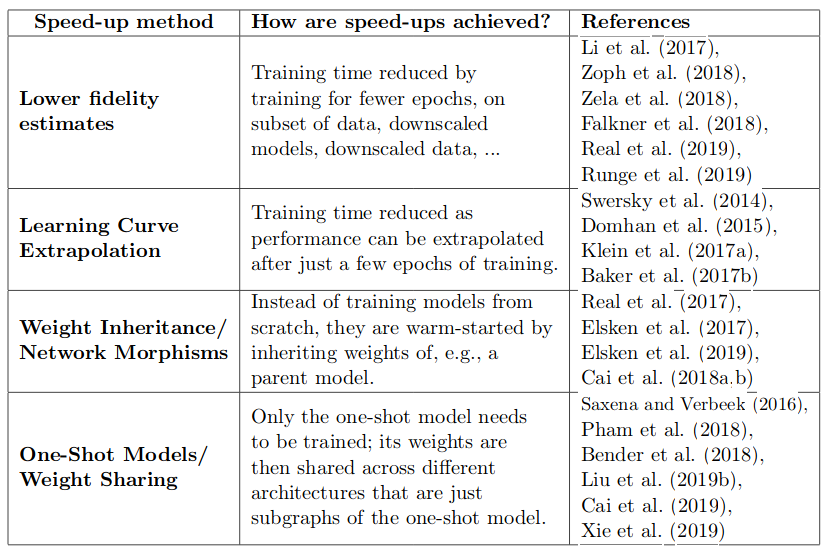
\includegraphics[width=0.9\textwidth]{images_lec7/performance_estimation.png}\\
\end{frame}
%----------------------------------------------------------------------



%----------------------------------------------------------------------
\myframe{Learning Goals}{

	After this lecture, you will be able to \ldots
	
	\begin{itemize}
		\item describe \alert{several ways of speeding up over blackbox NAS}  %(except via meta-learning)
		\myit{
			\item define \alert{network morphisms} \& \alert{explain how to use them to speed up NAS}
			\item explain various \alert{methods for extrapolating learning curves}
			\item explain various \alert{multi-fidelity Bayesian optimization methods}
		}
		\item discuss \alert{when and how to use NAS and HPO in practice} 
		\myit{
			\item describe \alert{failure modes of DARTS}
			\item describe \alert{Auto-DispNet}
		} 
		\item describe \alert{NAS-Bench-101}, a benchmark for NAS
	\end{itemize}
}


%-----------------------------------------------------------------------
\section{Network Morphisms and Weight Inheritance}
%-----------------------------------------------------------------------


%----------------------------------------------------
\begin{frame}{Network Morphisms}
    \begin{itemize}
    	\item \alert{Network Morphisms} \lit{Chen et al. ‘16; Wei et al. ‘16; Cai et al. ‘17}
	\begin{itemize}
		\item[--] \alert{Change the network structure, but not the modelled function}
		\item[--] i.e., for every input the network yields the same output as before applying
		the network morphisms 
		
		\item[--] Example operations: ``Net2DeeperNet'', ``Net2WiderNet'', etc.
	\end{itemize}
    \end{itemize}

    \begin{figure}[t]
        \begin{centering}
            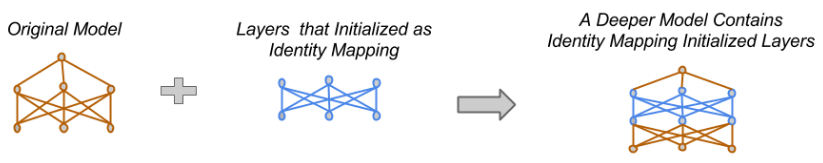
\includegraphics[scale=0.3]{images_lec7/net2deepernet.png}
        \end{centering}
    \end{figure}

\end{frame}

%----------------------------------------------------
\begin{frame}{Network Morphisms Allow Efficient Moves in Architecture Space}

    \begin{figure}[t]
        \begin{centering}
            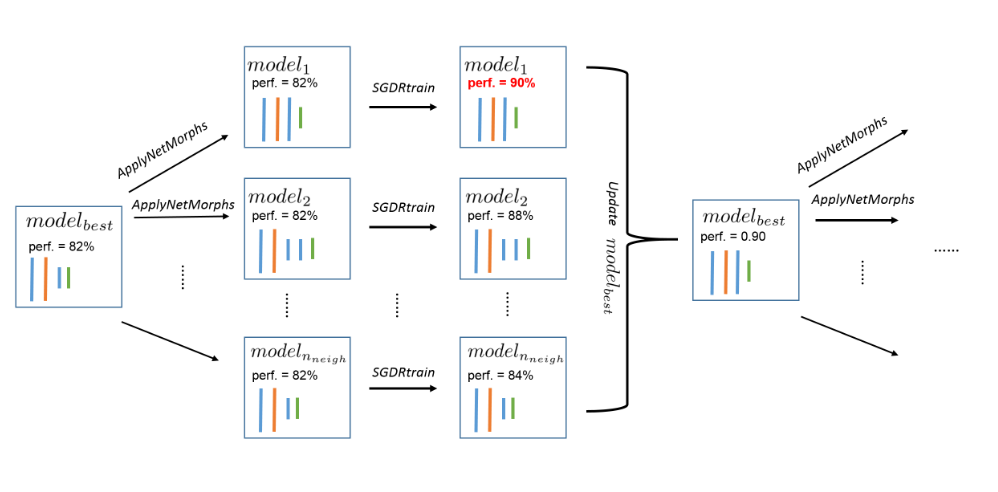
\includegraphics[scale=0.3]{images_lec7/NASH.png}
        \end{centering}
    \end{figure}


	%\alert{Weight Inheritance} 
	\lit{Real et al. ‘17; Cai et al, '17; Elsken et al, '17; Cai et al. ‘18; Elsken et al. ‘19}

\end{frame}
%----------------------------------------------------

%----------------------------------------------------
\begin{frame}{Efficient Multi-objective NAS \litw{Elsken et al. ‘19}}

{\small\alert{LEMONADE}: Lamarckian Evolution for Multi-Objective Neural Arch. Design}
    \begin{itemize}
    	\item Maintain a \alert{Pareto front} of the \alert{2 or more objectives}
    	\myit{
			\item Evolve a population of Pareto-optimal architectures over time
		}
		\item Use \alert{weight inheritance}
		\myit{
			\item[--] Inherit already trained weights from parent architectures to child ones
			\item[--] Allow \alert{approx.\ network morphisms} (function not preserved perfectly)
			\item[--] Still cheap through weight inheritance (e.g., 1 week on 8 GPUs)
    	}

    \end{itemize}
\vspace*{-0.1cm}
    \begin{figure}[t]
        \begin{centering}
            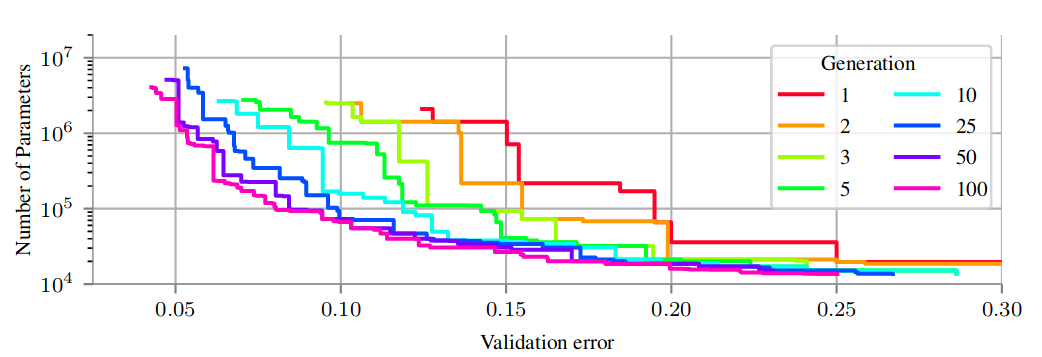
\includegraphics[scale=0.3]{images_lec7/lemonade.png}
        \end{centering}
    \end{figure}

\end{frame}
%----------------------------------------------------


%----------------------------------------------------

\begin{frame}[c]{Efficient Multi-objective NAS \litw{Elsken et al. ‘19}}
\begin{itemize}
	\item Children generation and training/evaluation of architectures 
\end{itemize}

\begin{centering}
    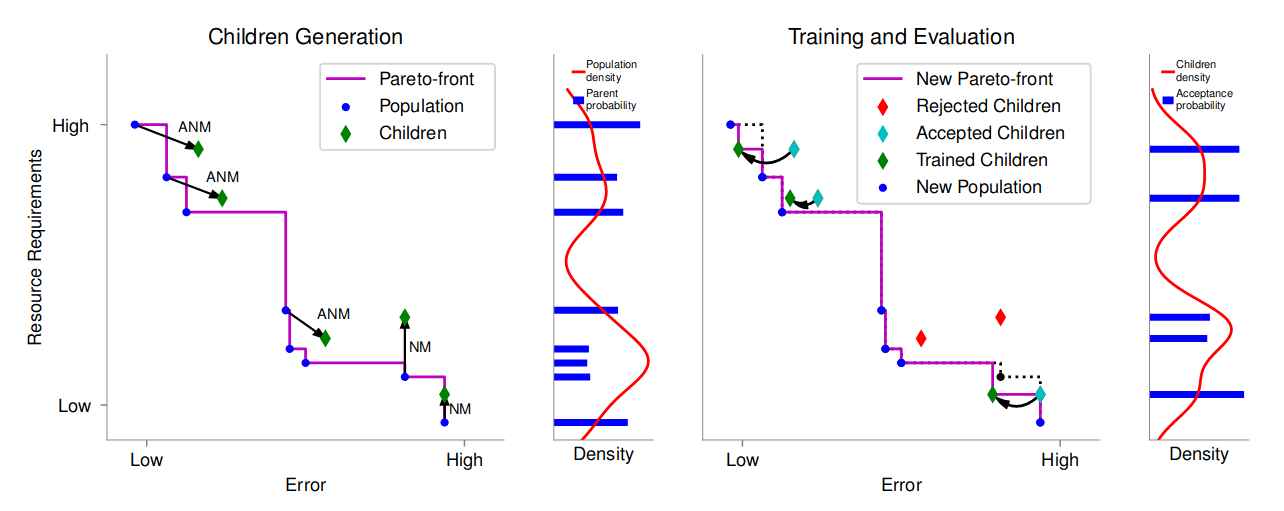
\includegraphics[scale=0.27]{images_lec7/lemonade_2.png}
\end{centering}

	\pause
	\myit{
			\item[--] \alert{Possible project: apply LEMONADE to SeizureNet}
			\item[--] \alert{Possible project: apply LEMONADE to algorithmic fairness}
			\item[--] \alert{Possible project: apply LEMONADE to adversarial robustness}
	}

\end{frame}

%----------------------------------------------------




%-----------------------------------------------------------------------
\section{Graybox Optimization: Learning Curve Extrapolation}
%----------------------------------------------------------------------

%-----------------------------------------------------------------------
\begin{frame}[c,fragile]{Learning Curves}

\centering
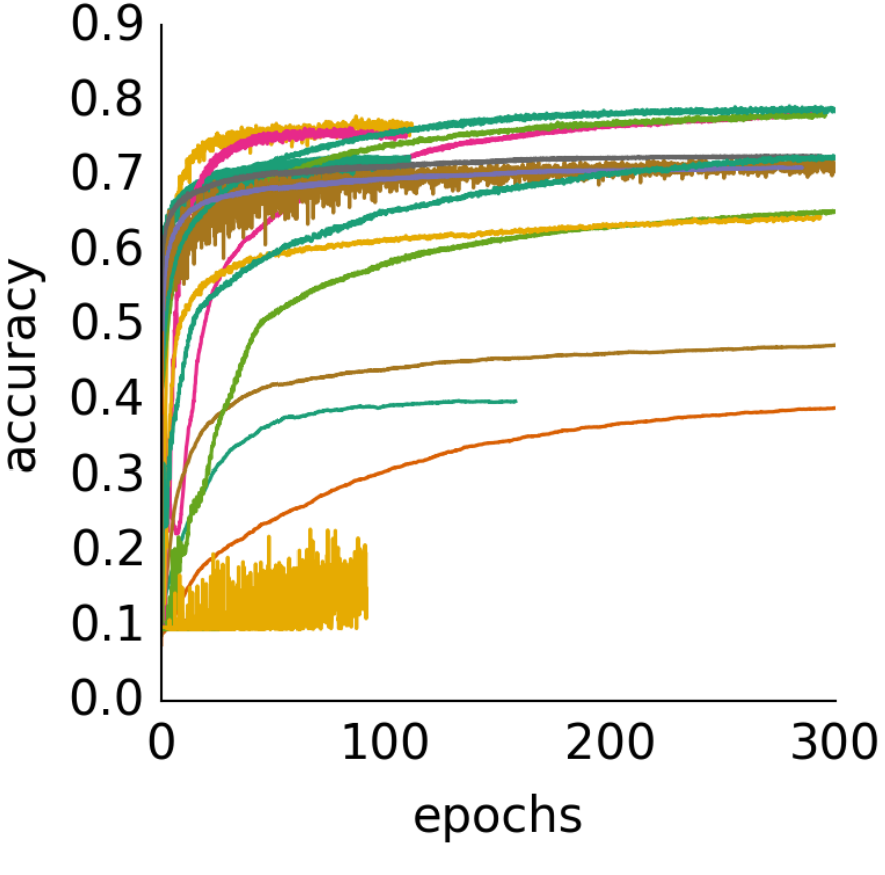
\includegraphics[width=0.5\textwidth]{images/learning_curves}

Exemplary learning curves of training deep neural networks\\
Many ML algorithms iteratively optimize a (loss) function

\end{frame}
%-----------------------------------------------------------------------

%-----------------------------------------------------------------------
\begin{frame}[c,fragile]{Learning Curve Predictions}

\centering
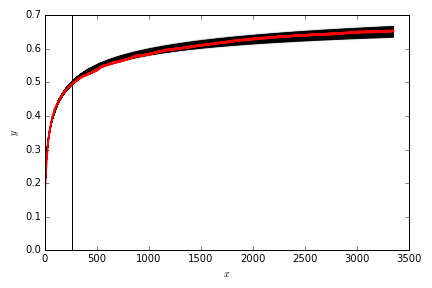
\includegraphics[width=0.6\textwidth]{images/learning_curve_single_pred}

\begin{enumerate}
  \item Observe learning curve for the first $n$ steps (here $n=250$)
  \pause
  \item \alert{Extrapolation}: fit parametric model on partial learning curve to predict remaining learning curve
  \pause
  \item Various models can be used (see following slides)
 % Which model to use? E.g.,
 % \begin{itemize}
%	\item Parametric density models: give table with equations
%	\item Neural network with learning curve layer
%	\item Recurrent neural network
%%    \item Good model depends on shape of curve $\to$ e.$\,$g., depends on optimizer  
%%    \item[$\leadsto$] combination of several models
%  \end{itemize}
  
\end{enumerate}

\end{frame}
%-----------------------------------------------------------------------

%-----------------------------------------------------------------------
\begin{frame}[c,fragile]{Learning Curves: Early Termination}

\centering
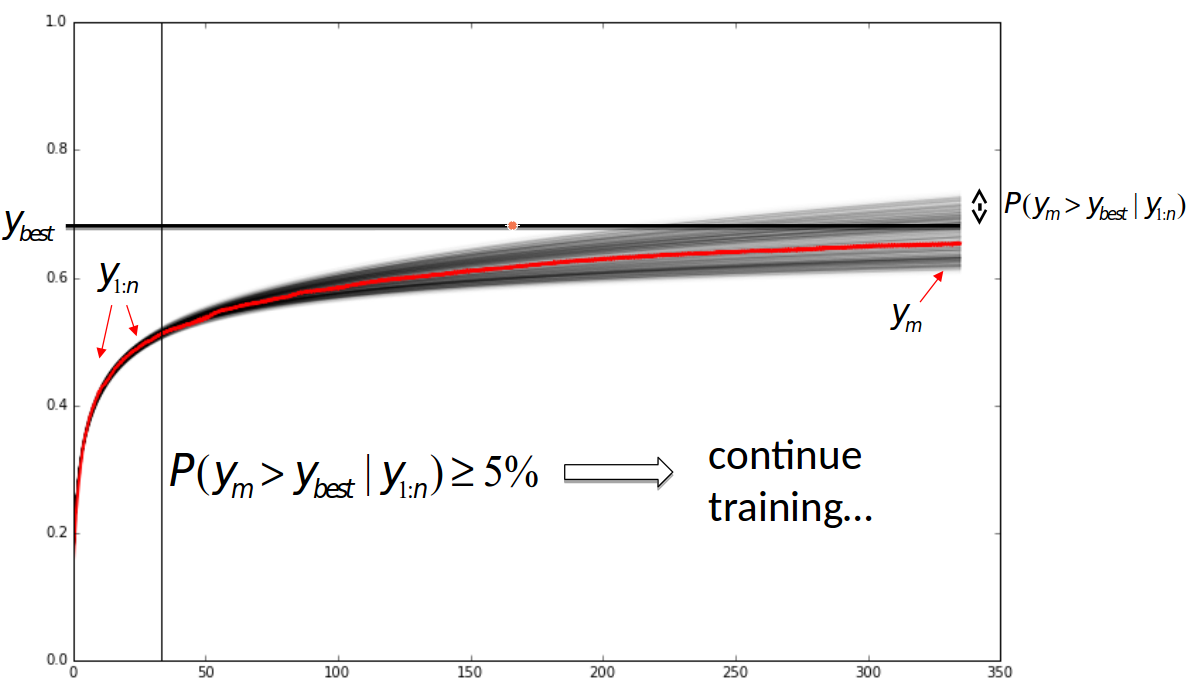
\includegraphics[width=\textwidth]{images/learning_curve_dec}

$\rightarrow$ need for \alert{probabilistic predictions / quantification of uncertainty}

\end{frame}
%-----------------------------------------------------------------------
%-----------------------------------------------------------------------
\begin{frame}[c,fragile]{Learning Curves: Early Termination}

\centering
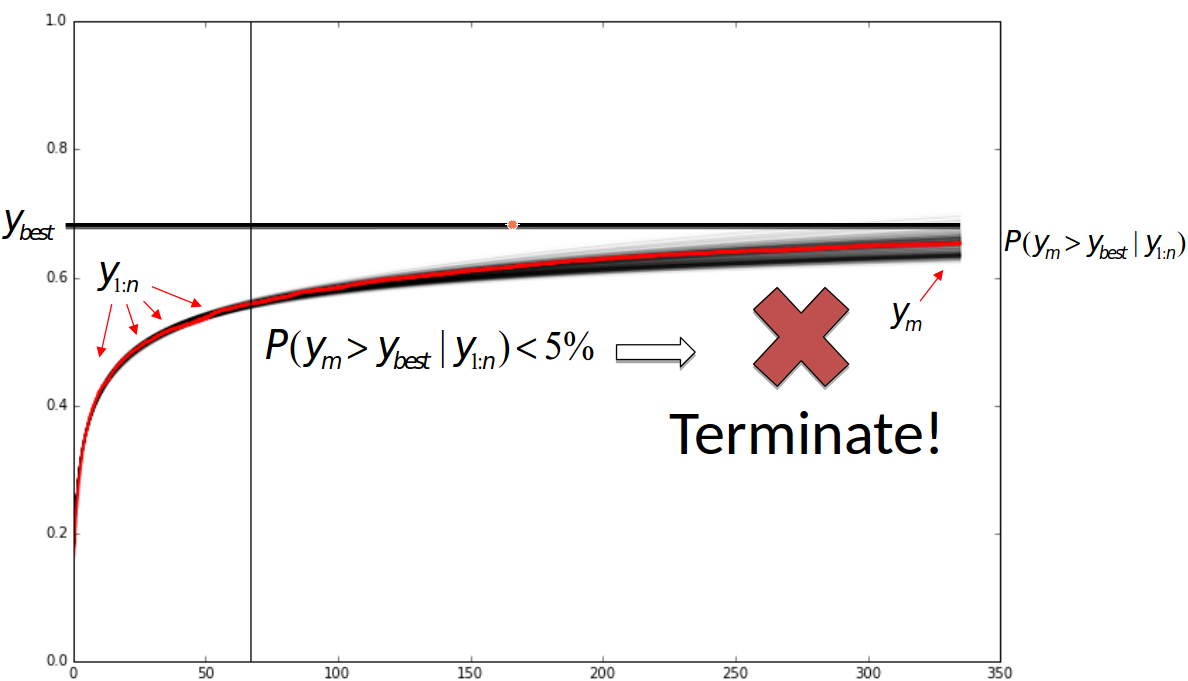
\includegraphics[width=\textwidth]{images/learning_curve_dec2}

$\rightarrow$ need for \alert{probabilistic predictions / quantification of uncertainty}

\end{frame}
%-----------------------------------------------------------------------

%-----------------------------------------------------------------------
\begin{frame}[c,fragile]{Domhan et al, 2015: Parametric Learning Curves}

\myit{
	\item Use a parametric model $f_k$ with parameters $\boldsymbol{\theta}$ to model performance at step $t$ as:
	\alert{$y_t = f_k(t|\boldsymbol{\theta}) + \epsilon$}, with $\epsilon \sim \mathcal{N}(0, \sigma^2)$.
\pause
	\item Linear combination of $K=11$ parametric types of models:
	\alert{$f_{comb}(t|\bm{\xi}) = \sum_{k=1}^K w_k f_k(t|\boldsymbol{\theta}_k)$},
where $\bm{\xi} = (w_1, \dots, w_{K}, \boldsymbol{\theta}_1, \dots, \boldsymbol{\theta}_{K}, \sigma^2)$
%	\item MSc Thesis in my group, 2015
}
\begin{center}
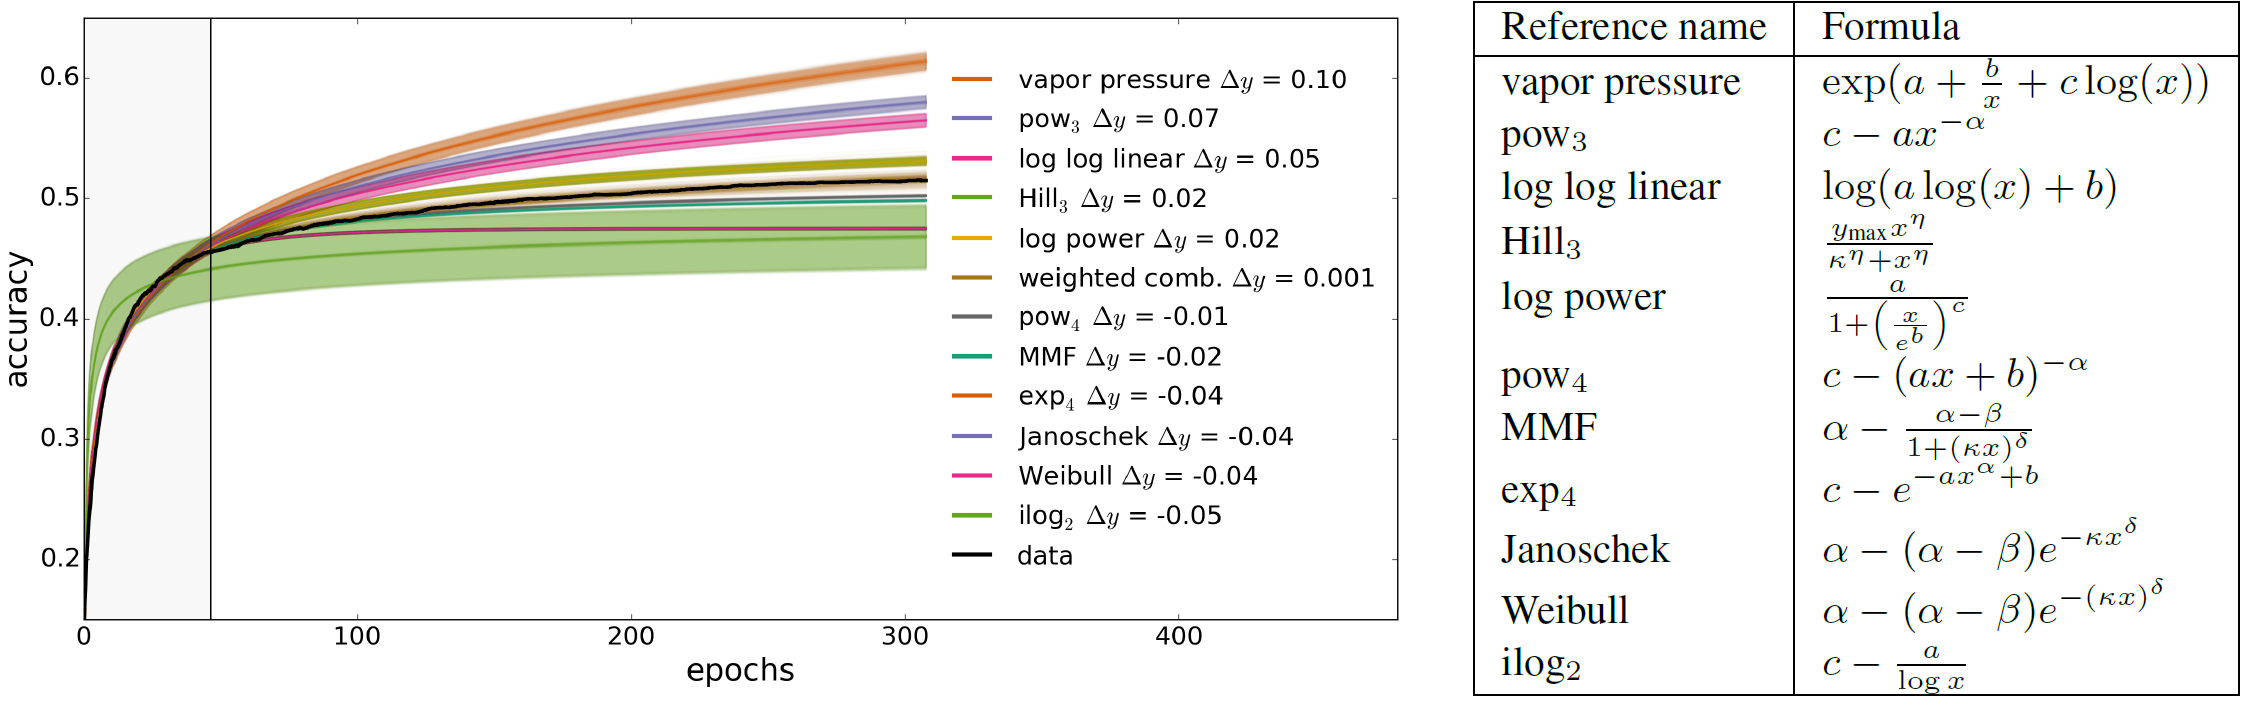
\includegraphics[width=0.9\textwidth]{images_lec8/Domhan_types_of_curves.png}\\
\scriptsize{$K=11$ parametric families for modelling learning curves}
\end{center}

\pause
\myit{
	\item Use Markov Chain Monte Carlo sampling of $\bm{\xi}$ to obtain uncertainties
}

\end{frame}
%-----------------------------------------------------------------------

%-----------------------------------------------------------------------
\begin{frame}[c,fragile]{Predictive Termination by Domhan et al, 2015}

{
\begin{center}
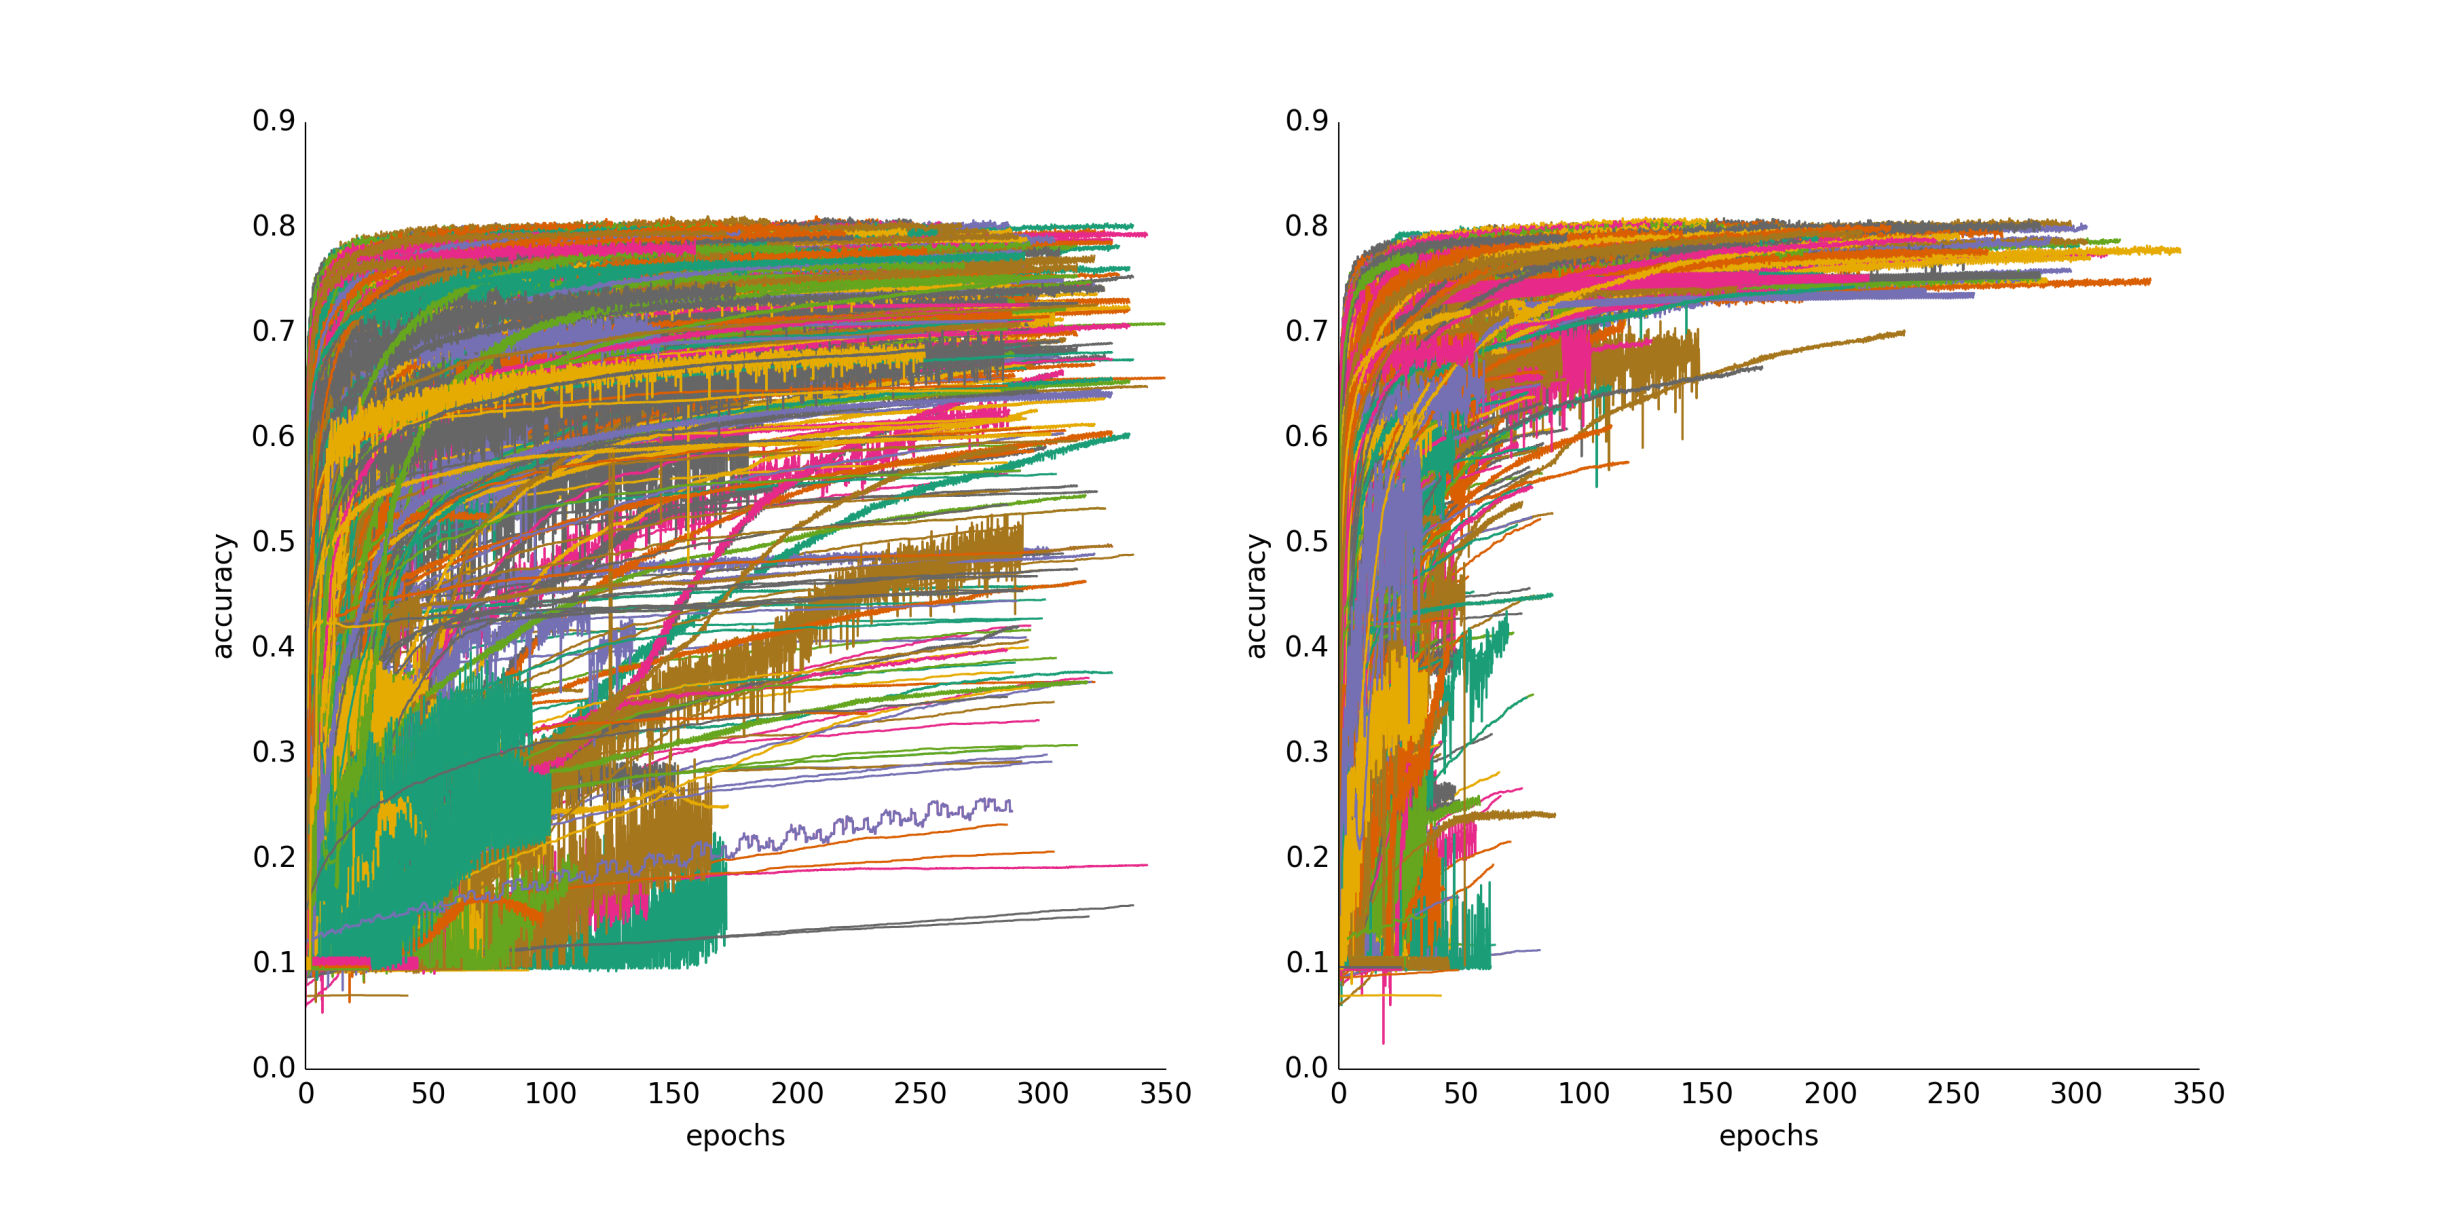
\includegraphics[width=0.7\textwidth]{images/learning_curve_tuning}

All learning curves vs. learning curves with early termination
\end{center}
}
\pause

\myit{
	\item Disadvantages of this model? 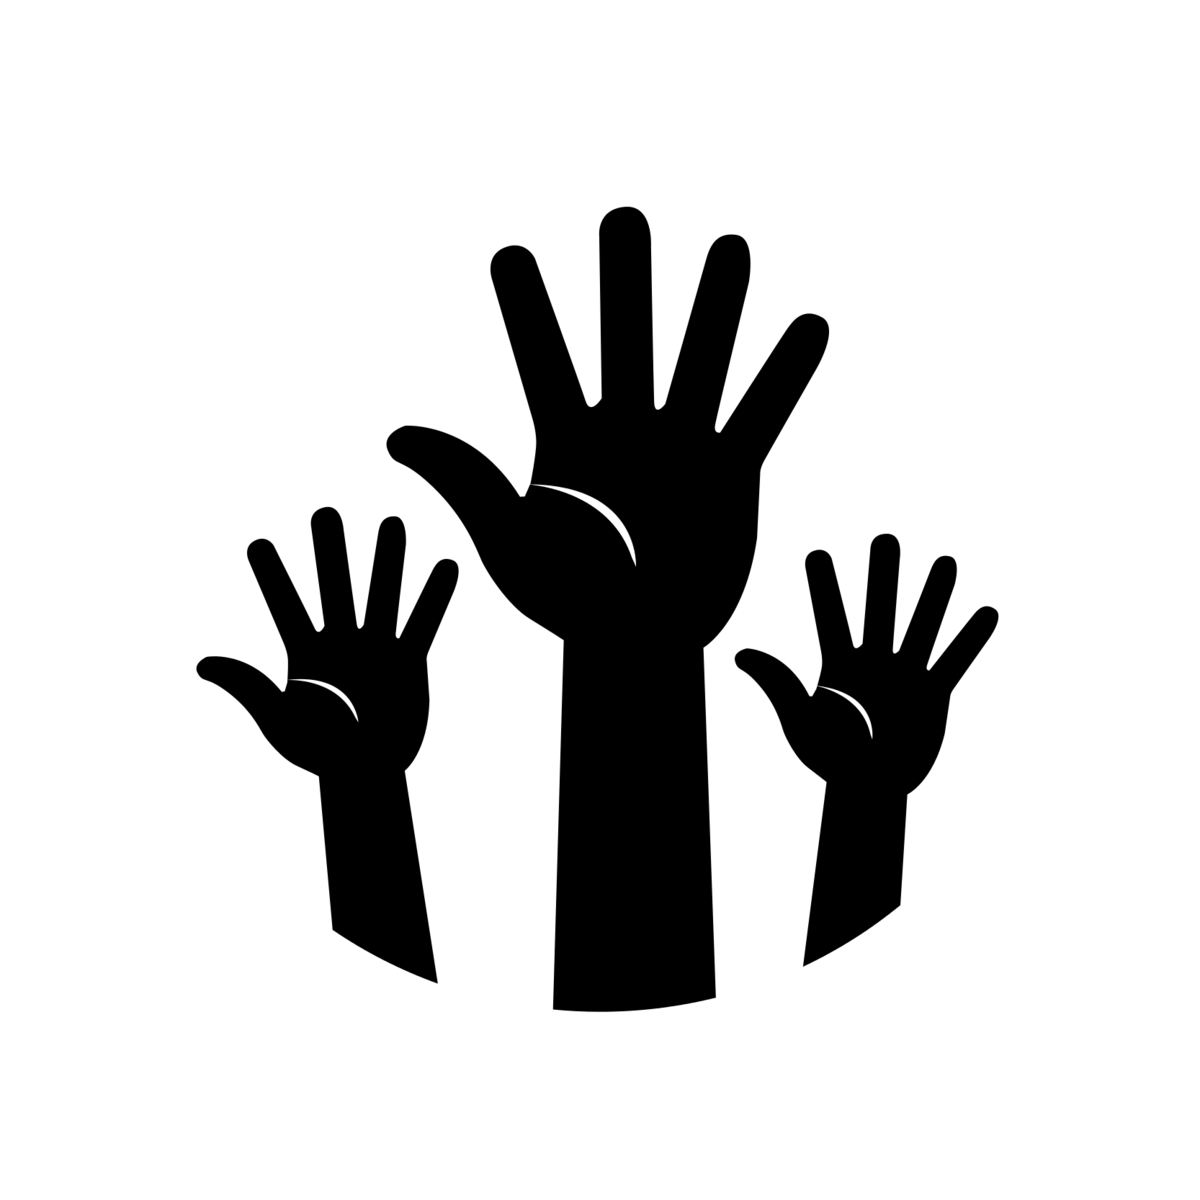
\includegraphics[height=0.08\textheight]{images/hands.png}
\pause
	\myit{
		\item Relies on manually-selected parametric families of curves
		\item Does not take into account hyperparameters used 
		\myit{
			\item[$\rightarrow$] can't learn across hyperparameters
		}
		\item Does not even learn across curves; simply extrapolates one at a time
%		\item Cannot quickly integrate new information from extending the curve
	}
}

\end{frame}
%-----------------------------------------------------------------------


%-----------------------------------------------------------------------
\begin{frame}[c,fragile]{Freeze-Thaw Bayesian Optimization (Swersky et al, 2014)}

\myit{
	\item Use a Gaussian process with inputs $\conf$ and $t$; special kernel for $t$
	\item For $N$ configurations and $T$ epochs each: $O(N^3 t^3)$ $\rightarrow$ approximation
	\item Iteratively: either extend existing configuration or try new one
\pause
	\item Result for probabilistic matrix factorization:
	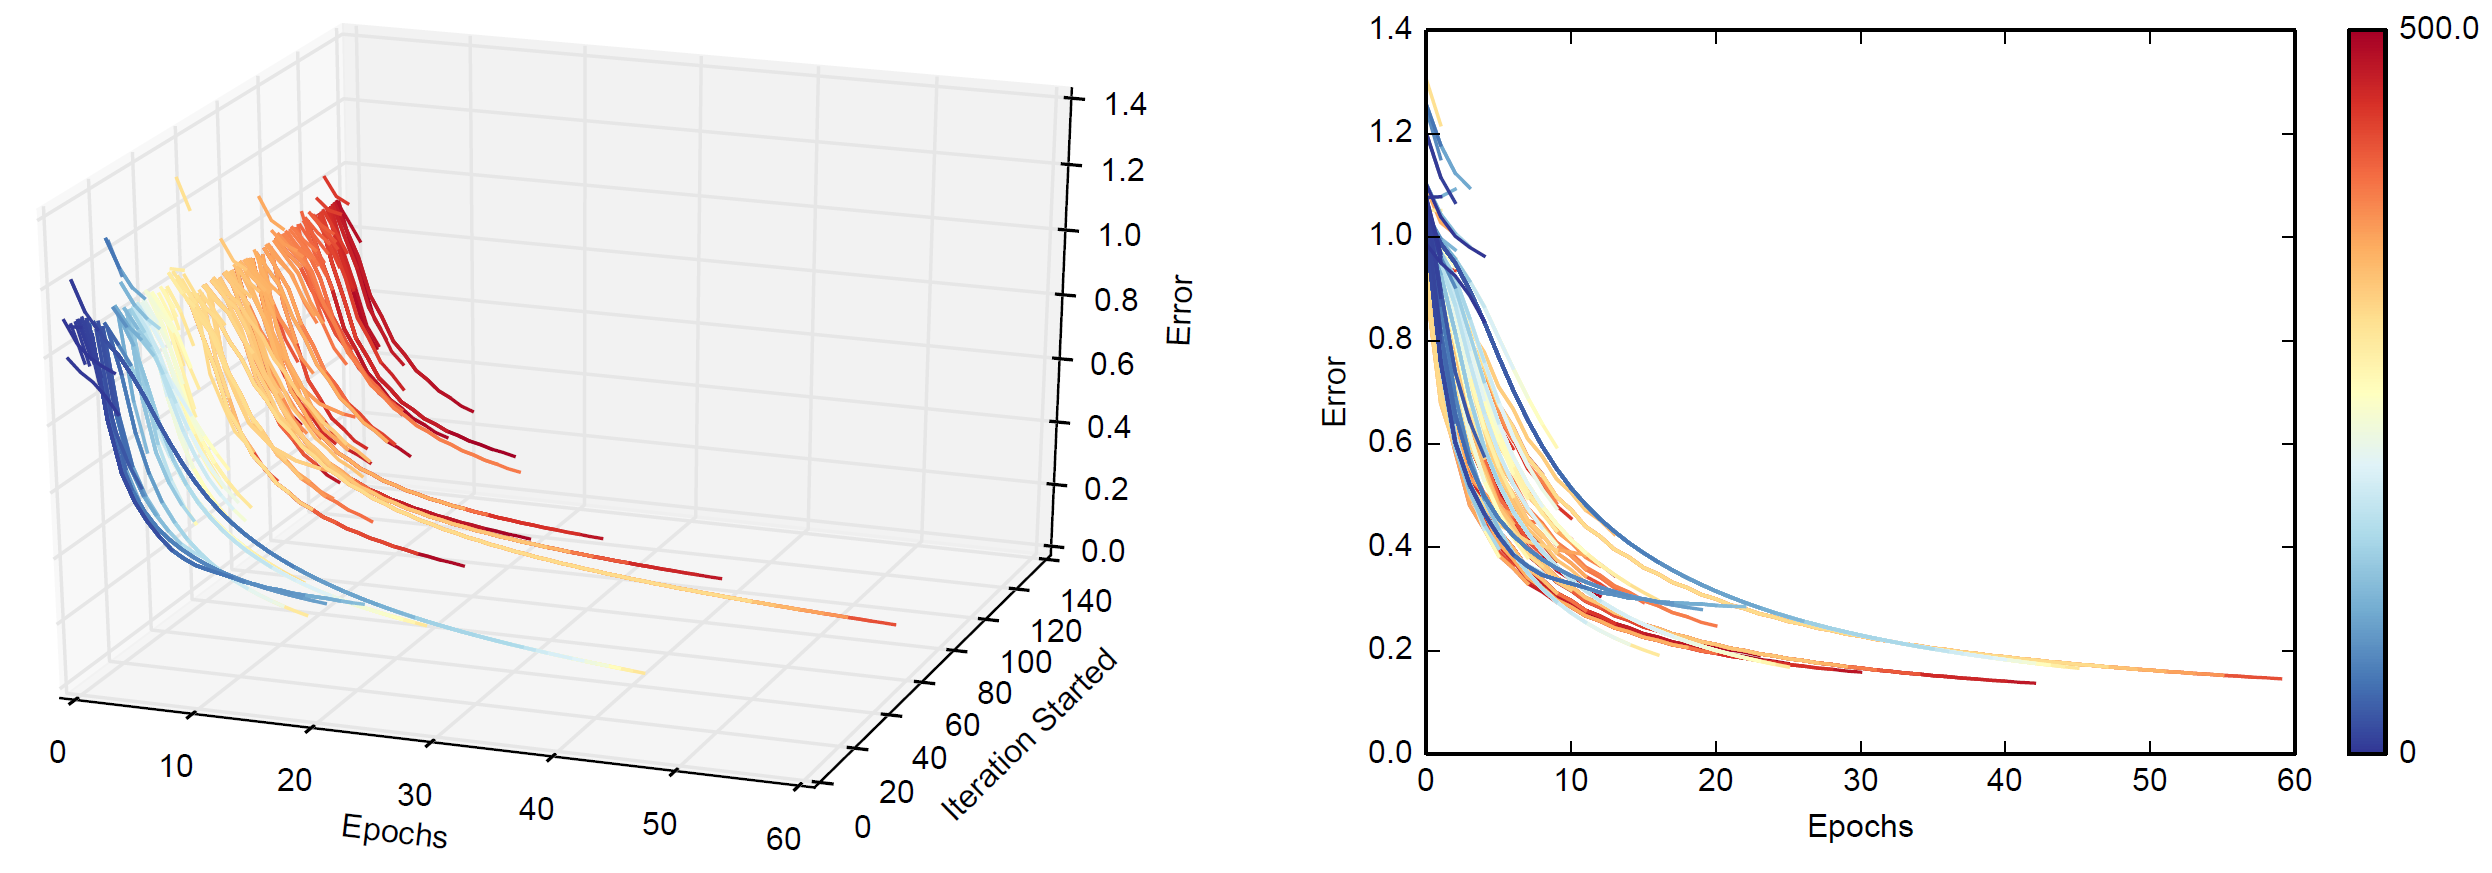
\includegraphics[width=0.8\textwidth]{images_lec8/FTBO}
\pause
	\item Unfortunately, no results for DNNs; no code available
}


\end{frame}
%-----------------------------------------------------------------------


%-----------------------------------------------------------------------
\begin{frame}[c,fragile]{Klein et al, 2017: LC-Net}

\vspace*{-0.5cm}
{
	\rightimage[.4]{images_lec8/LC-Net-network.png}
	\myit{
		\item \goleft[.45]{Make a layer out of the parametric learning curves by Domhan et al.}
		\item \goleft[.45]{Also support hyperparameters as inputs (in the figure denoted by $x_1, \dots, x_d$)}
%		\item \goleft[.45]{Work by my Phd student Aaron Klein and postdoc Stefan Falkner}
	}
}

\pause
\myit{
	\item Disadvantages of this model? 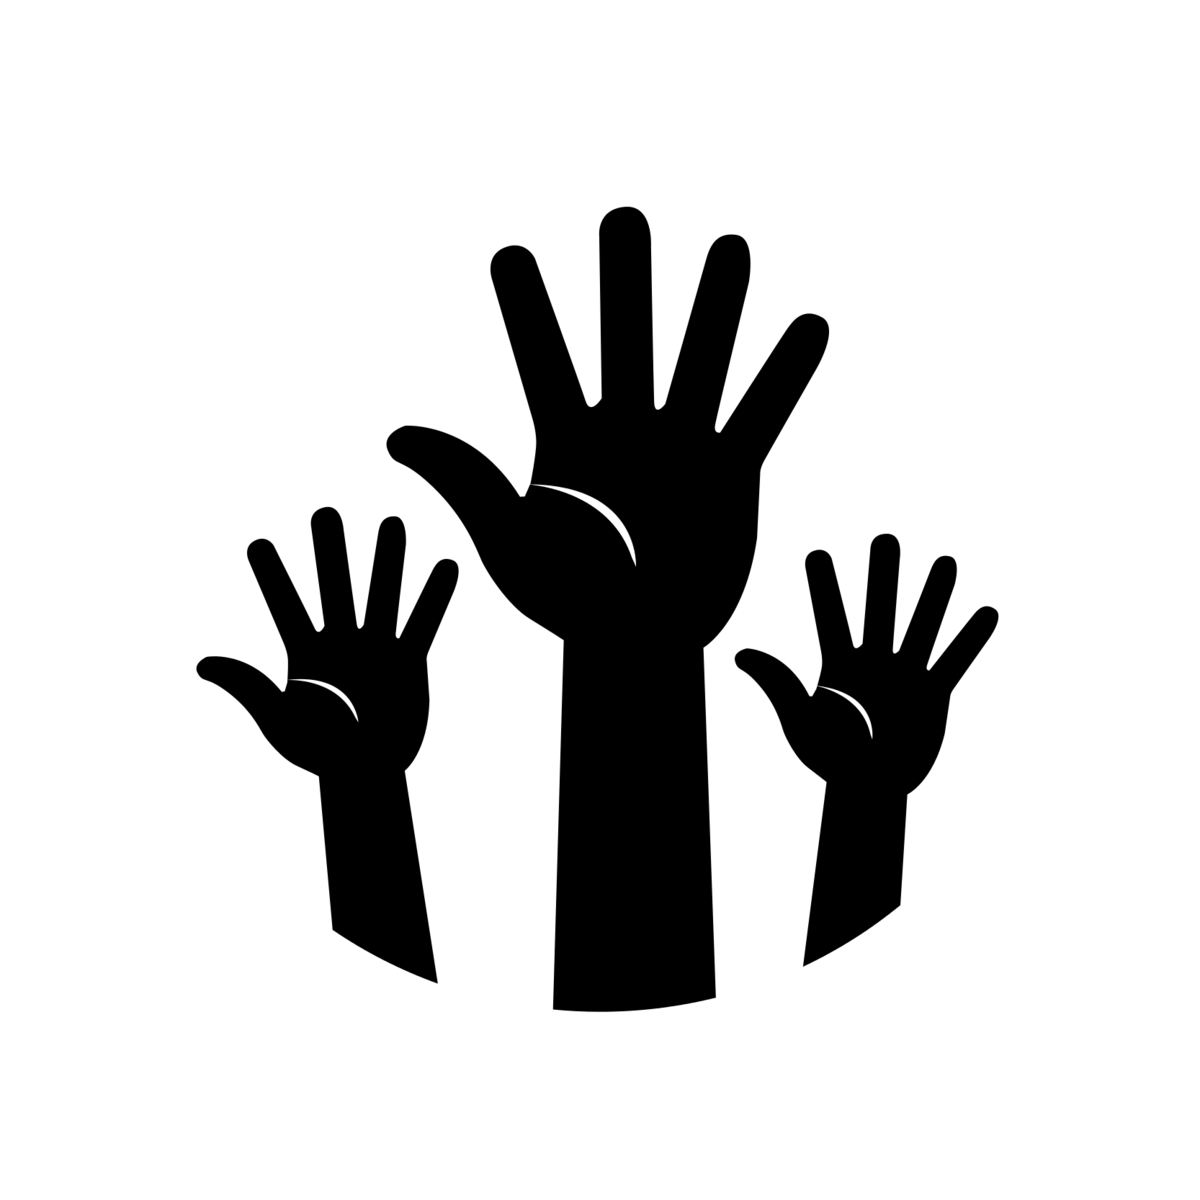
\includegraphics[height=0.1\textheight]{images/hands.png}
	\pause
	\myit{
		\item \goleft[.45]{Relies on manually-selected parametric families of curves}
		\item \goleft[.45]{Cannot quickly integrate new information from extending the current curve \\ (or from new runs)}
	}
}
\end{frame}
%-----------------------------------------------------------------------



%-----------------------------------------------------------------------
\begin{frame}[c,fragile]{Gargiani et al, 2019: Sequence Models {\smaller{(e.g., Bayesian RNN)}}}

	\myit{
		\item Learning curves are \alert{sequences}
		\myit{
			\item Previous models don't treat them like this
			\item We can use an RNN (in particular, an LSTM) to predict the next value from a given sequence
			\item We can use variational dropout to obtain uncertainty estimates:
\pause
		}
	}
\vspace*{-0.5cm}
\begin{center}
	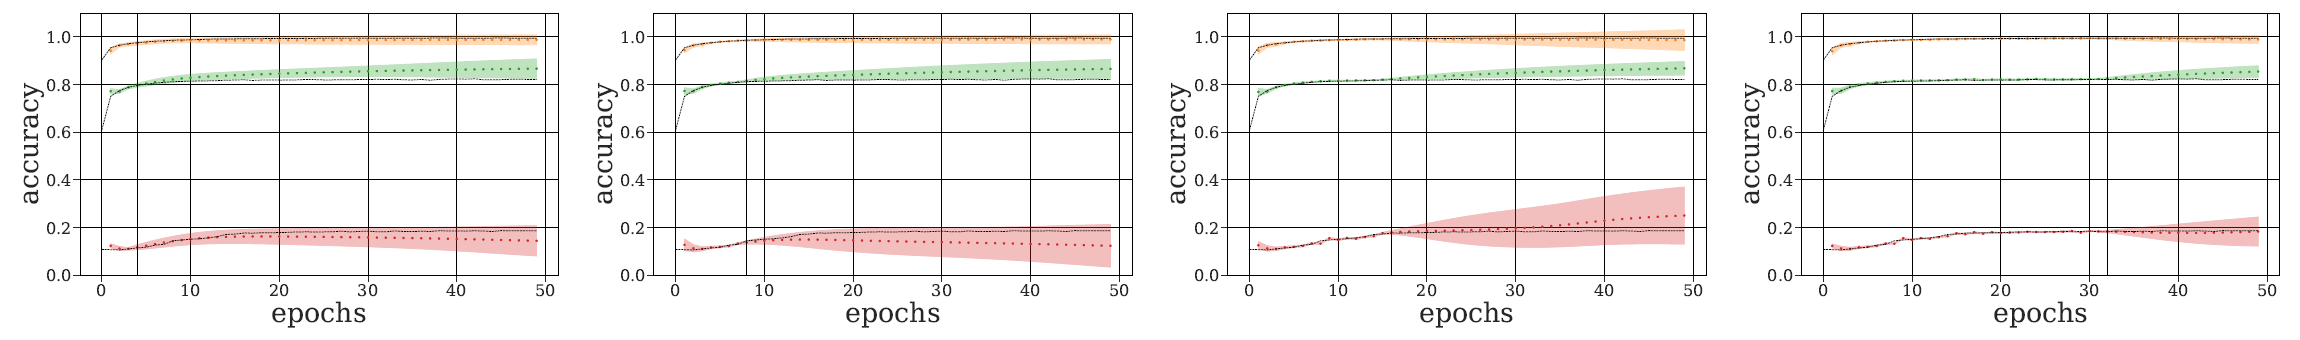
\includegraphics[height=0.2\textheight]{images_lec8/Gargiani-MNIST-extrapolations}\\
\end{center}	
	\myit{
		\item Note: we can also use a simpler model
		\myit{
			\item E.g., a random forest to map from a fixed-size window to the next value
		}
	}
\vspace*{-0.25cm}
\begin{center}
	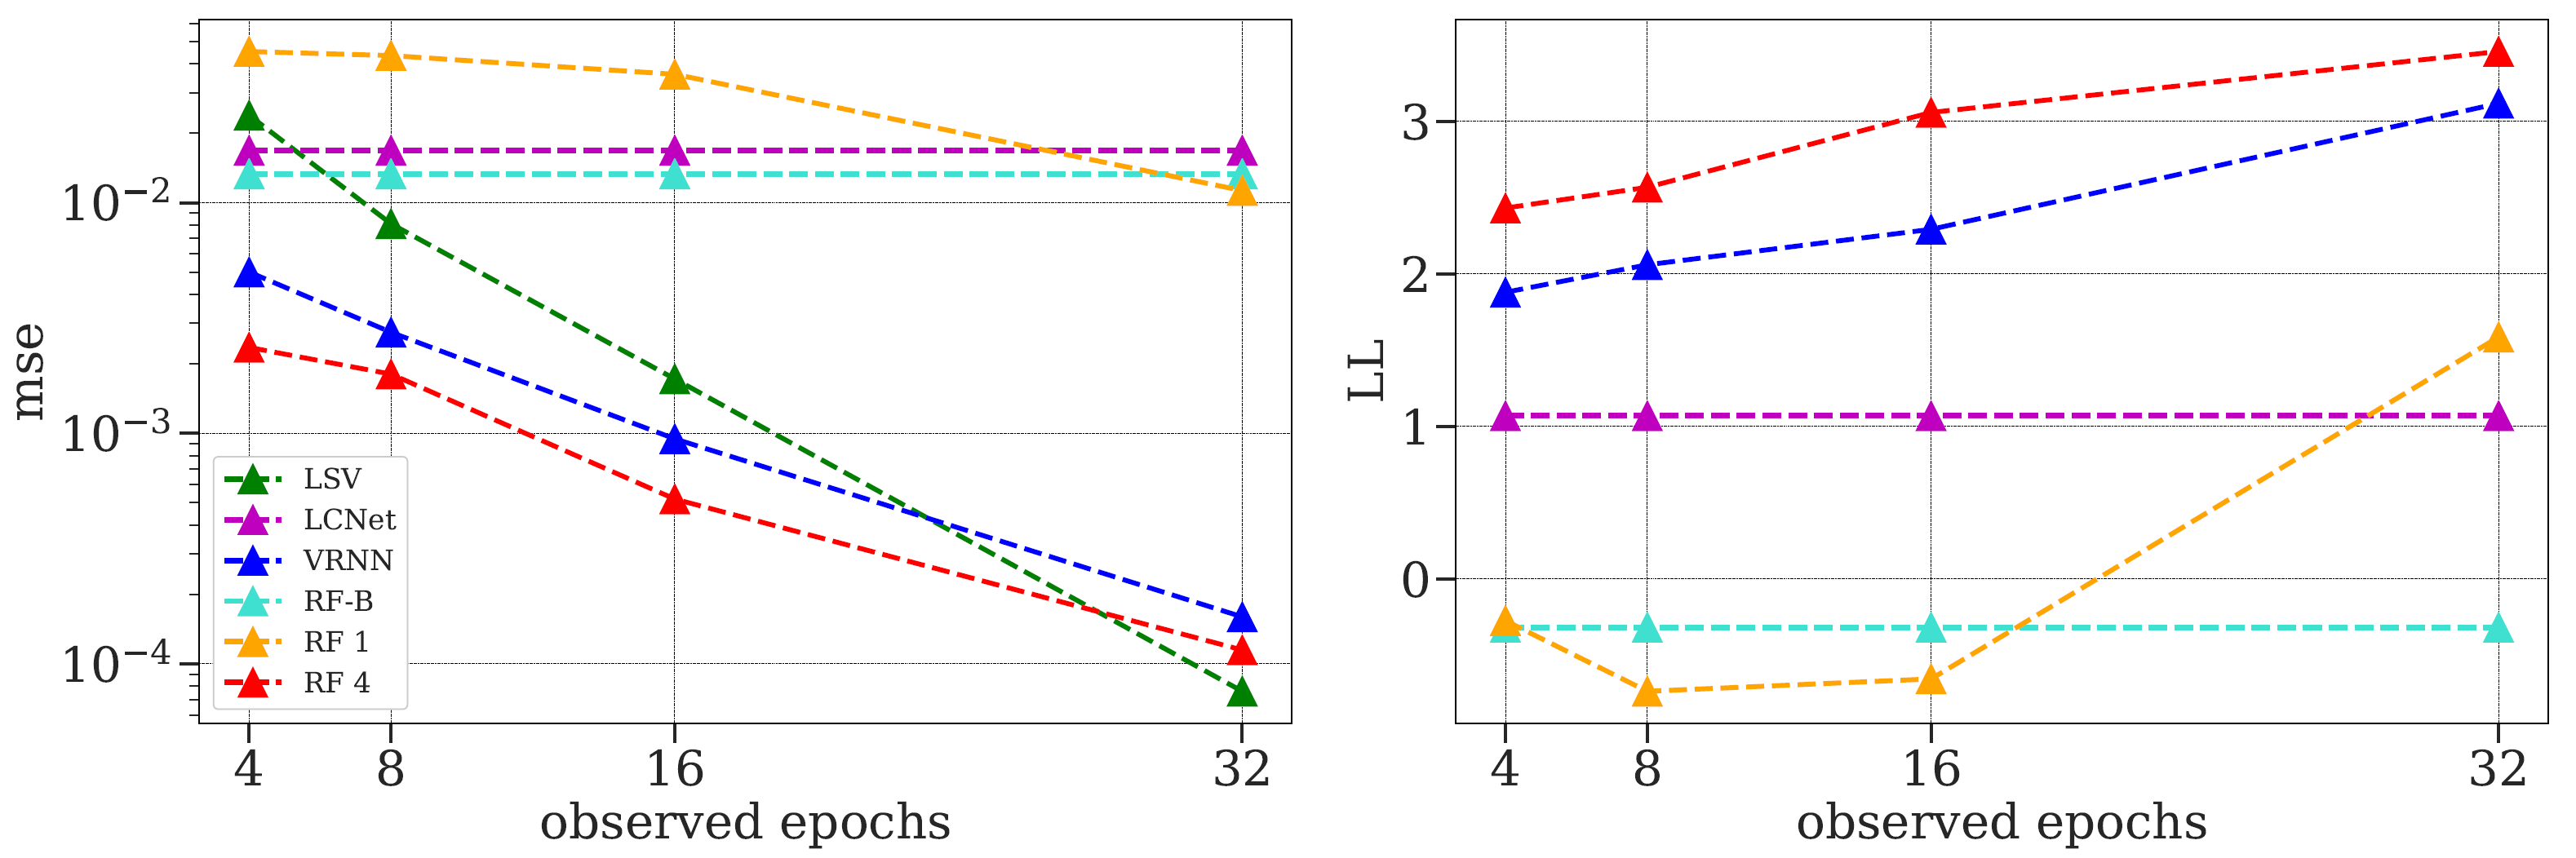
\includegraphics[height=0.2\textheight]{images_lec8/Gargiani-MNIST-extrapolation-quality-based-on-different-sized-prefixes}
\end{center}	
\end{frame}
%-----------------------------------------------------------------------

%-----------------------------------------------------------------------
\begin{frame}[c,fragile]{Compare: Baker et al, 2017}

	\myit{
		\item Idea: Map from configurations (including architectural hyperparameters) 
		and partial learning curves to the final performance

		\item Advantages
		\myit{
			\item \alert{Much simpler idea} than all the approaches just discussed: no need to model the entire learning curve
			\item \alert{Much easier to implement}
		}
		\item Disadvantage? \pause
		\alert{$\rightarrow$ requires many (e.g., 100) fully-evaluated learning curves as training data}
		\myit{
			\item After 100 full function evaluations we want to be pretty much converged in practice
			\item But definitely helpful for speeding up RL
			\item Can be combined with Hyperband and be used whenever we have enough runs for a budget
		}
	}

%Describe simple idea, and how that works extremely well when you have a budget of 10.000 of function evaluations.

\end{frame}
%-----------------------------------------------------------------------


\myframe{Possible extension of LC models waiting to be done}{
	\myit{
		\item We could keep track of additional information to feed to our model for better predictions
		\myit{
			\item E.g., training \& validation cross-entropy loss \& accuracy
			\myit{
				\item Instead of only validation accuracy
			}
			\item E.g., split cross-entry into data-dependent \& weight dependent parts
			\item E.g., keep track of gradient norms, activation statistics, \ldots
		}
		\item Information about learning rate (\& weight decay) at each step
		\item[$\rightarrow$] possible student project
	}
}





%-----------------------------------------------------------------------
\section{Graybox Optimization: Using Multiple Fidelities}
%----------------------------------------------------------------------

%-----------------------------------------------------------------------
\myframe{Motivating Example}{
	\myit{
		\item Performance of an SVM on MNIST and subsets of it:\\~\\
%		    \item Computational cost grows quadratically in dataset size $s$
%		\item 
	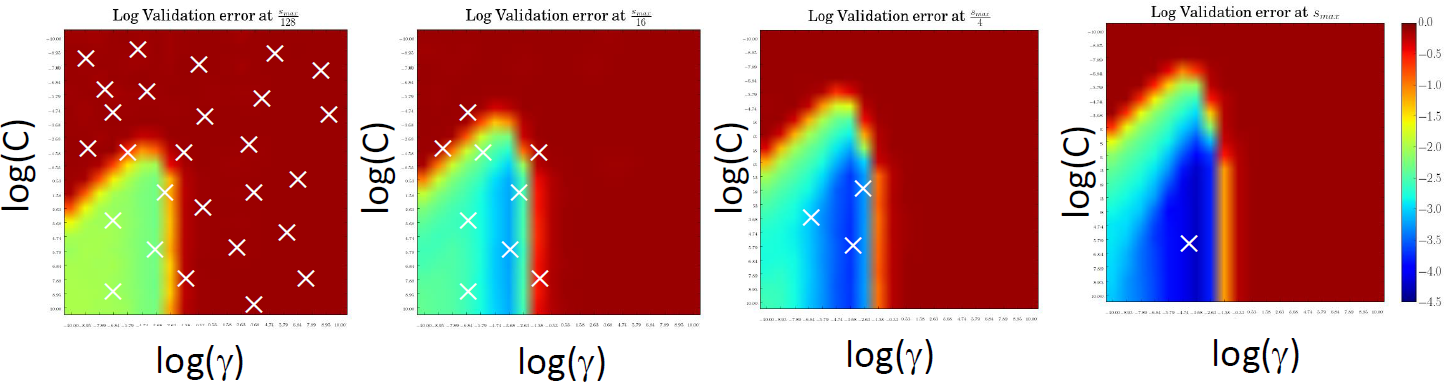
\includegraphics[width=0.9\textwidth]{images/hyperparameter_optimization/MNIST.png} 
		\item Evaluations on the smallest subset (128 data points) cost 10\,000 less than on the full data set
	}
}

%-----------------------------------------------------------------------
\myframe{Multifidelity Optimization}{
	\myit{
		\item Use \alert{cheap approximations of the expensive blackbox}, performance on which correlates with the blackbox, e.g.
		\myit{
			\item Subsets of the data
			\item Fewer epochs of iterative training algorithms (e.g., SGD; DARTS)
			\item Shorter MCMC chains in Bayesian deep learning
			\item Fewer trials in deep reinforcement learning
			\item Downsampled images in object recognition
			\item Shallower networks
		}
		\pause
		\medskip
		\item \alert{Also applicable in different domains}, e.g., fluid simulations:
		\myit{
			\item Less particles
			\item Shorter simulations
		}
		\pause
		\item Possible project (Arber has already been looking into this): \\
		using multiple fidelities to find best setting of DARTS
	}
}
%-----------------------------------------------------------------------


%-----------------------------------------------------------------------
\myframe{One approach for handling multiple fidelities}{
	\myit{
		\item \alert{Multi-fidelity Bayesian optimization} for fidelity with values $b\in B$ %is the number of epochs for SGD $t\in \mathds{N^+}$
		\item Standard Bayesian optimization uses a model $f(\conf) \approx y$ to select the next $\conf$
		\item \alert{Multi-fidelity Bayesian optimization} uses a model $f(\conf\alert{, b}) \approx y$ to select the next $(\conf\alert{, b})$
\pause
		\myit{
			\item Model $f$ needs to be good at extrapolating from small to large $b$
			\item E.g., a learning curve model 
			\myit{
				\item When the budgets are different numbers of epochs for SGD
			}
			\item E.g., a Gaussian process for extrapolating from small to large datasets
			\myit{
				\item 1\,000-fold speedups for SVM on MNIST example \lit{\href{proceedings.mlr.press/v54/klein17a/klein17a.pdf}{Klein et al, AISTATS 2017}}
				\item This was based on \alert{Entropy Search}
			}
		}
	}	
}
%-----------------------------------------------------------------------


%%%%%%%%%%%%%%%%%%%%%%%%%%%%%%%%%%%%%%%%%%%%%%%%%%%%%%%%%%%%%%%%%%%%%%%%%
\myframe{Refresher: Entropy Search}{
	\myit{
		\item Define the $p_{\text{min}}$ distribution given data $\mathcal{D}$:
		$$p_{\text{min}}(x' \mid \alert{\mathcal{D}}) := p(x' \in \argmin_{x\in X} f(x) \mid \alert{\mathcal{D}})$$
	
		\item Entropy search aims to minimize the entropy \alert{$H[p_\text{min}]$} 
		\item In a nutshell:
		\begin{enumerate}
			\item Estimate $p(f \mid \mathcal{D})$, e.g., using a GP (as before)
			\item Approximate $p_\text{min}$ by representer points and Monte-Carlo simulations
%			\item Compute entropy $H[p_{\text{min} \mid \mathcal{D}]$
			\item Select $x$ that minimizes the following acquisition function:
		\end{enumerate}
	}
\vspace*{0.5cm}
	\[a_{\text{ES}}(x) := \mathds{E}_{\alert{p(y\mid x, \mathcal{D})}} 
	\left[   H[p_{\text{min}}(\cdot \mid \alert{\mathcal{D} \cup \{(x, y)\}})] \right]\]
}
%%%%%%%%%%%%%%%%%%%%%%%%%%%%%%%%%%%%%%%%%%%%%%%%%%%%%%%%%%%%%%%%%%%%%%%%%

%%%%%%%%%%%%%%%%%%%%%%%%%%%%%%%%%%%%%%%%%%%%%%%%%%%%%%%%%%%%%%%%%%%%%%%%%
\myframe{Multi-fidelity Bayesian Optimization with Entropy Search}{
	\myit{
		\item We care about the $p_{\text{min}}$ distribution for the maximal budget $B$:
		$$p_{\text{min}}(x' \mid \mathcal{D}) := p(x' \in \argmin_{x\in X} f(x\alert{,B}) \mid \mathcal{D})$$
	
		\item We still want to minimize the entropy $H[p_\text{min}]$
\pause
		\item Now we aim for the biggest \alert{reduction in entropy per time spent}
		\myit{
			\item Next to $f$, we \alert{now also model the cost $c(x,b)$}
			\item We choose the next $(x,b)$ by maximizing:
		}
	}
\vspace*{0.5cm}
	\[a_{\text{ES}}(x,b) := \mathds{E}_{\alert{p(y\mid (x, b), \mathcal{D})}} 
	\left[   \frac{H[p_{\text{min}}(\cdot \mid \alert{\mathcal{D}})] - H[p_{\text{min}}(\cdot \mid \alert{\mathcal{D} \cup \{((x,b), y)\}})]}{\alert{c(x,b)}} \right]\]

}

%%%%%%%%%%%%%%%%%%%%%%%%%%%%%%%%%%%%%%%%%%%%%%%%%%%%%%%%%%%%%%%%%%%%%%%%%


%%%%%%%%%%%%%%%%%%%%%%%%%%%%%%%%%%%%%%%%%%%%%%%%%%%%%%%%%%%%%%%%%%%%%%%%%
\myframe{Multi-fidelity Bayesian Optimization with Entropy Search}{
	\myit{	
		\item The entire algorithm iterates the following 2 steps until time is up:
		\begin{enumerate}
			\item Select $(x,b)$ by maximizing:
			\[a_{\text{ES}}(x,b) := \mathds{E}_{\alert{p(y\mid (x, b), \mathcal{D})}} 
	\left[   \frac{H[p_{\text{min}}(\cdot \mid \alert{\mathcal{D}})] - H[p_{\text{min}}(\cdot \mid \alert{\mathcal{D} \cup \{((x,b), y)\}}]}{\alert{c(x,b)}} \right]\]
			\item Observe performance and cost, and update models $f$ and $c$ 
		\end{enumerate}

\pause
\vspace*{0.2cm}		
		\item Pros:
		\myit{
			\item Conceptually beautiful
			\item 1\,000-fold speedups for optimizing SVMs on MNIST
		}
		\item Cons:
		\myit{
			\item \alert{Scalability} of GPs is a big problem (limits size of initial design)
			\item \alert{Limited applicability of Gaussian processes}
		}
	}
}

%%%%%%%%%%%%%%%%%%%%%%%%%%%%%%%%%%%%%%%%%%%%%%%%%%%%%%%%%%%%%%%%%%%%%%%%%
 
%-----------------------------------------------------------------------
\myframe{Related works}{
	\myit{
		\item Similar ways to attack the same problem
		\myit{	
			\item First choose $x$ based on \alert{UCB}, then choose $b$ afterwards\\ \lit{\href{http://papers.nips.cc/paper/6117-gaussian-process-bandit-optimisation-with-multi-fidelity-evaluations}{Kandasamy et al, 2016}; \href{https://arxiv.org/abs/1703.06240}{Kandsamy et al, 2017}}
			\item Use the \alert{knowledge gradient} acquisition function instead of entropy search \lit{\href{https://arxiv.org/abs/1903.04703}{Wu et al, 2019}}
			\item Use the efficient \alert{max-value entropy search} instead of standard entropy search \lit{\href{https://arxiv.org/abs/1901.08275}{Takeno et al, 2019}}
\pause
			\item Possible project: compare these empirically
		}
\vspace*{0.2cm}
\pause
		\item More scalable models
		\myit{
			\item Bayesian optimization with Bayesian neural networks \lit{\href{https://papers.nips.cc/paper/6117-bayesian-optimization-with-robust-bayesian-neural-networks}{Springenberg et al, 2016}}; but not yet evaluated for the multi-fidelity case 
		}
\pause
		\item Possible project: \alert{scalable model for the multi-multi-fidelity case} (or also some model-free approach)
	}
}
%-----------------------------------------------------------------------



%-----------------------------------------------------------------------
%\myframetop{Tree of Parzen Estimators (TPE) \footnotesize{[Bergstra et al., 2011]}}{
%\begin{columns}[T]
%\column{0.35\textwidth}
%		\myit{
%			\item non-parametric KDE for $p(\vec x)$ instead of Gaussian Processes modelling $p(y \vert \vec x)$
%			\item equivalent to expected improvement
%			\item[+] efficient $\mathcal{O}(N\cdot d)$
%			\item[+] complex search spaces with priors
%			\item[+] parallelizable
%			\item[-] not as sample efficient as GPs
%		}
%\column{0.64\textwidth}
%\only<1 | handout:1>{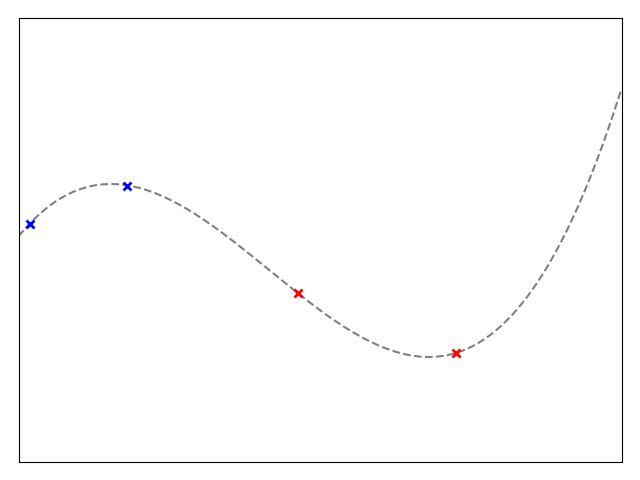
\includegraphics[width=0.95\linewidth]{./images/plots_aaron/iter_0_observations.png}}
%\only<2 | handout:2>{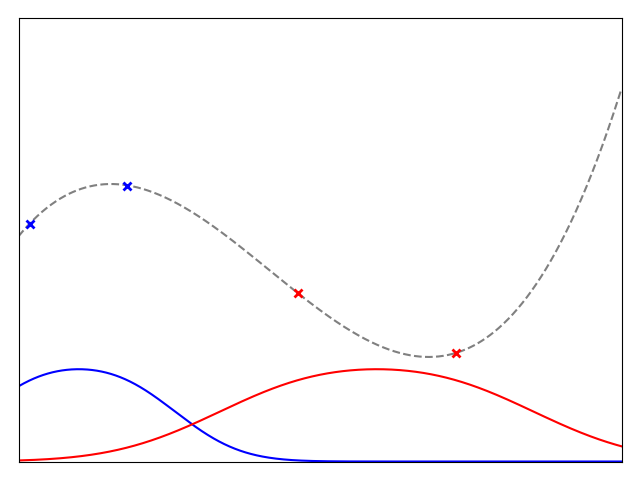
\includegraphics[width=0.95\linewidth]{./images/plots_aaron/iter_0_pdfs.png}}
%\only<3 | handout:3>{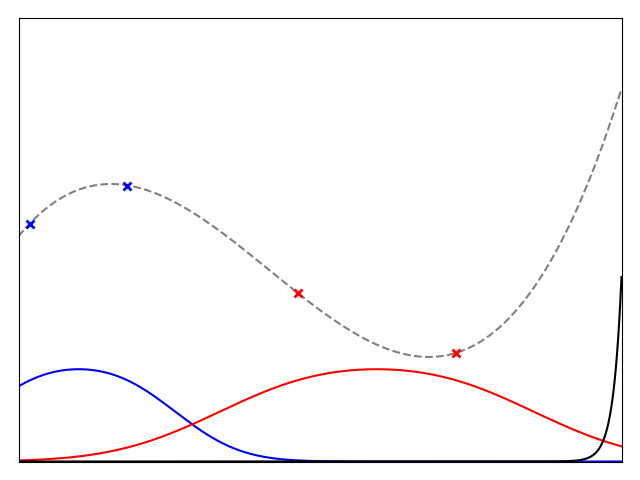
\includegraphics[width=0.95\linewidth]{./images/plots_aaron/iter_0_ei.png}}
%\only<4 | handout:4>{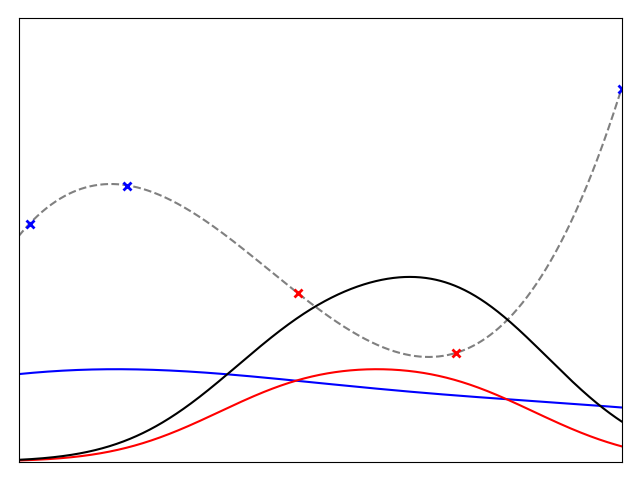
\includegraphics[width=0.95\linewidth]{./images/plots_aaron/iter_1_ei.png}}
%\only<5 | handout:5>{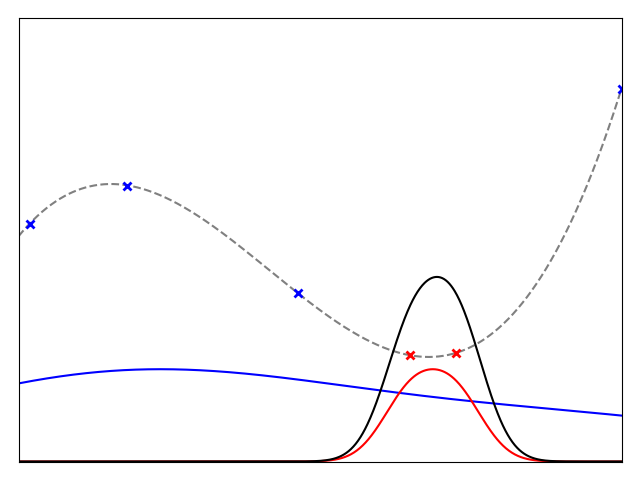
\includegraphics[width=0.95\linewidth]{./images/plots_aaron/iter_2_ei.png}}
%\end{columns}
%}
%%-----------------------------------------------------------------------

%-----------------------------------------------------------------------
\myframe{Can't we solve this problem more easily?}{
	\myit{
		\item Performance of an SVM on MNIST and subsets of it:\\~\\
	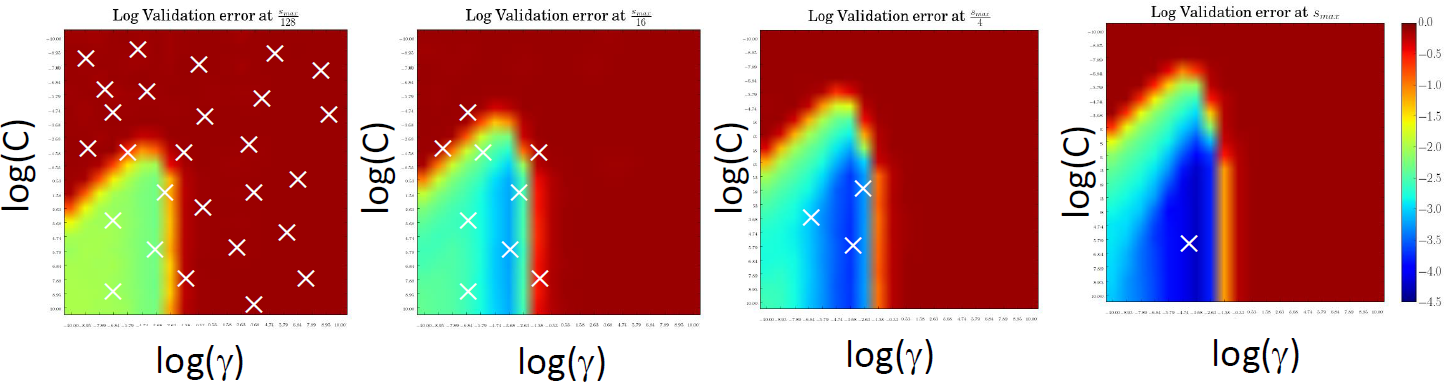
\includegraphics[width=0.9\textwidth]{images/hyperparameter_optimization/MNIST.png} 
		
		
		\item \alert{Successive Halving} \lit{\href{https://arxiv.org/pdf/1502.07943}{Jamieson \& Talwalkar, 2015}}
		\myit{
			\item Try a lot of random configurations on lowest budget
			\item Let best ones survive to next budget; iterate
		}
		\item This is surprisingly effective!
	}
}
%-----------------------------------------------------------------------

%-----------------------------------------------------------------------
\myframe{Successive Halving with a Wall Clock Time Budget}{
   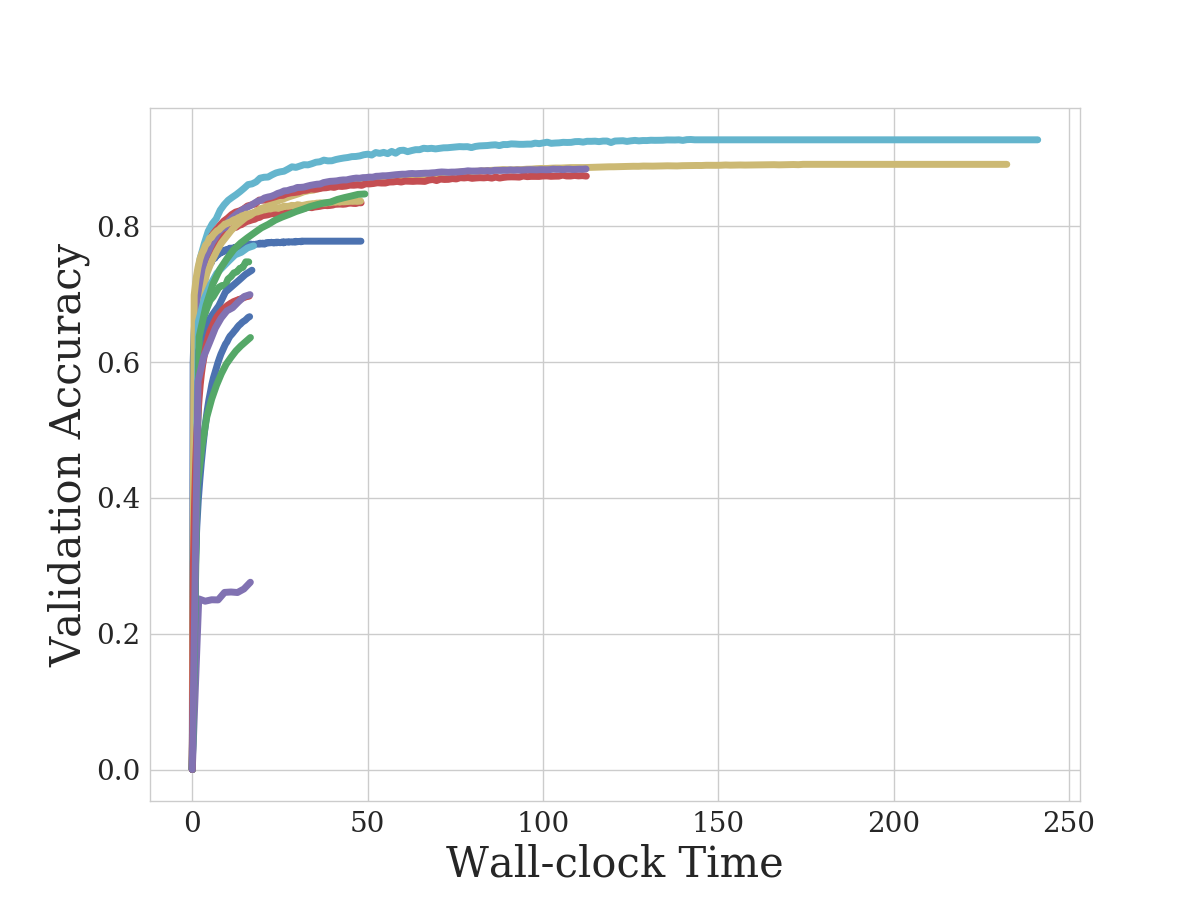
\includegraphics[width=.9\textwidth]{images/plots_aaron/successive_halving.png}
}
%-----------------------------------------------------------------------

%-----------------------------------------------------------------------
\myframe{Hyperband with a Wall Clock Time Budget: 4 iterations}{
  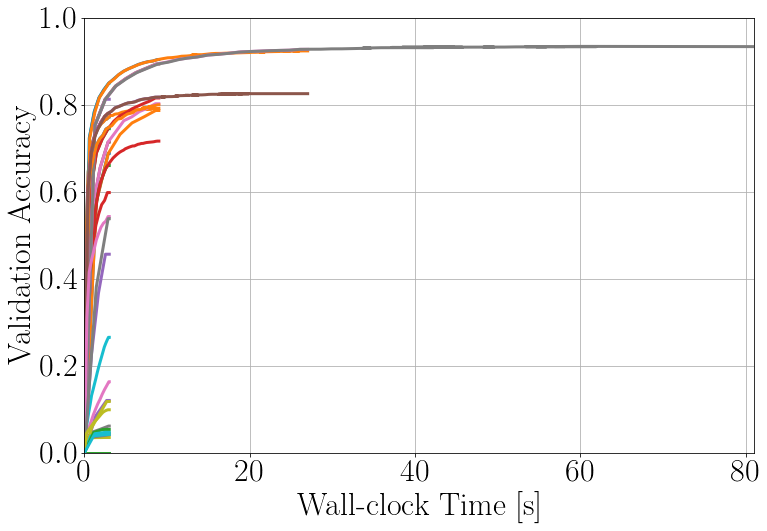
\includegraphics[width=.44\linewidth]{images/plots_aaron/hb_bracket_1.png}
  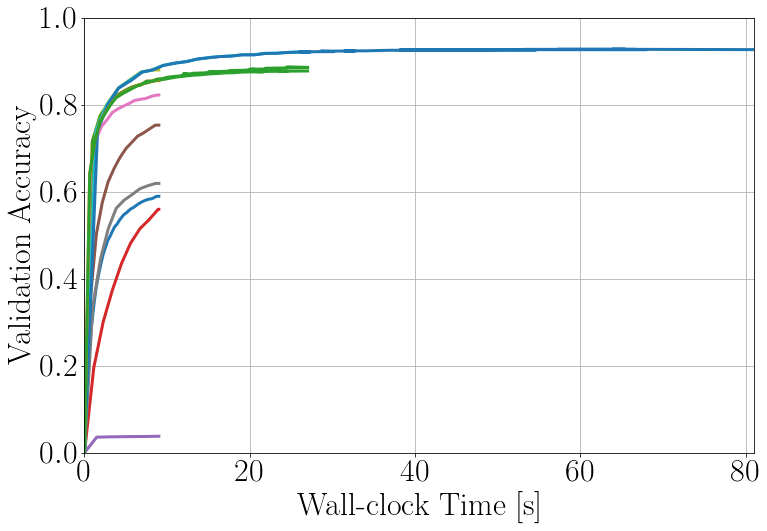
\includegraphics[width=.44\linewidth]{images/plots_aaron/hb_bracket_2.png}\\
  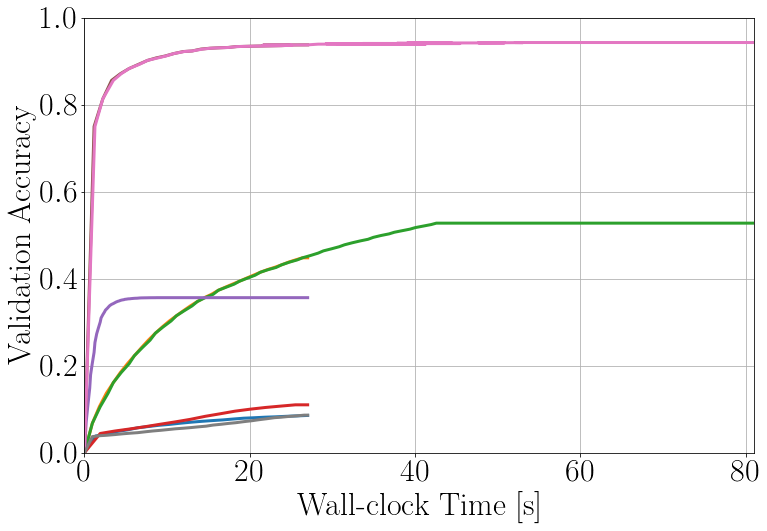
\includegraphics[width=.44\linewidth]{images/plots_aaron/hb_bracket_3.png}
  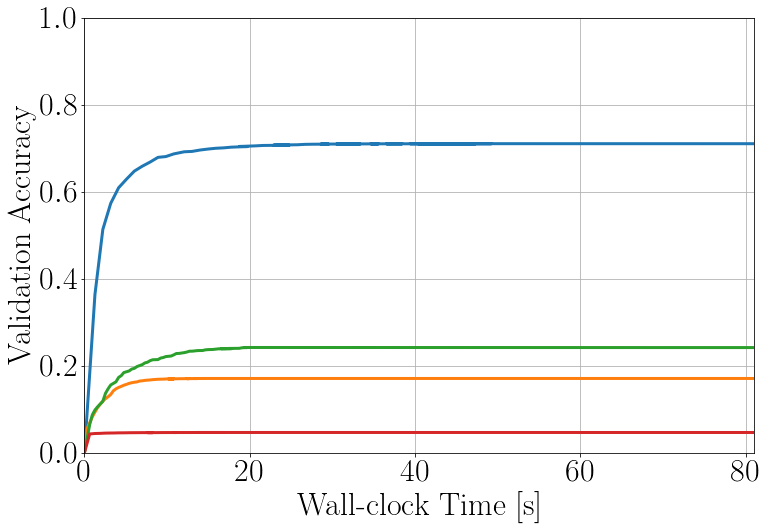
\includegraphics[width=.44\linewidth]{images/plots_aaron/hb_bracket_4.png}\\

	\begin{center}
	\lit{\href{https://openreview.net/forum?id=ry18Ww5ee}{Li et al, 2017}}
	\end{center}
}
%-----------------------------------------------------------------------

%-----------------------------------------------------------------------
\myframe{Hyperband}{
	%  \includegraphics[width=\linewidth]{plots/hb_pseudo_code.png}
	\begin{algorithm2e}[H]
		\caption{Pseudocode for Hyperband}
	        \DontPrintSemicolon
		\SetKwRepeat{Do}{do}{while}
	        \SetKwInOut{Input}{input}\SetKwInOut{Output}{output}
		\Input{budgets $b_{min}$ and $b_{max}$, $\eta$}
		$s_{max} = \lfloor \log_{\eta} \frac{b_{max}}{b_{min}} \rfloor + 1$ \tcp*{number of different iterations}
		
		\For{$s_i \in \{ s_{max}-1, s_{max}-2, \dots , 1, 0$ \}}{
			$n = \lceil \frac{s_{max}}{s_i+1}\cdot \eta^{s_i} \rceil$  \tcp*{number of initial configurations}
			$b = \eta^{-s_i}\cdot b_{max}$ \tcp*{initial budget}
			C = $\mathrm{sample\_random\_configurations}(n)$ \;
			\Do{$b_i \leq b_{max}$}{
				L = $\mathrm{map}(\mathrm{evaluate}, C, b)$\tcp*{run with budget $b$}
			$n_i = \lfloor n_i / \eta \rfloor$ \tcp*{ reduce number of configurations}
			$b_i = b_i \cdot \eta$\tcp*{increase their budget}
			$C = C[\mathrm{argsort}(L)[:n_i] ]$\tcp*{\small{keep best $\eta^{-1}$ of configs}}
			}
		\Return configuration or model with lowest loss
		}
	\end{algorithm2e}
}
%-----------------------------------------------------------------------



%-----------------------------------------------------------------------
\myframe{BOHB: Robust and Efficient Hyperparameter Optimization at Scale}{
  
	\myit{
		\item Simple Combination of Bayesian Optimization and HyperBand \\ \lit{\href{http://proceedings.mlr.press/v80/falkner18a.html}{Falkner et al, ICML 2018}}
		\myit{
			\item[-] Bayesian optimization for selecting configurations (a TPE-like variant)
			\item[-] Hyperband for selecting the budgets for them
			
		}
\pause
\medskip		
		\item Advantages 
		\myit{
			\item[-] \alert{Robust and efficient off-the-shelf tool} 
			\item[-] Strong anytime performance
			\item[-] Strong performance with larger budgets 
			\item[-] Scalable to high dimensions, parallel workers, different parameter types (categorical, integer, continuous) 
			\item[-] \alert{On Github: \url{https://github.com/automl/HpBandSter}}
%			\item[-] New, so only 50 stars 
		}

\pause
\medskip		
		\item To the best of my knowledge, still the best available tool 
		\item \alert{Many possible projects around BOHB -- better models, multi-multi-fidelity, etc}

	}
}
%-----------------------------------------------------------------------


\myframe{How BOHB chooses the next configuration}{
\begin{algorithm2e}[H]
%\begin{algorithm2e}[b]
	\caption{BOHB: choose configuration}
        \DontPrintSemicolon
        \SetKwInOut{Input}{input}\SetKwInOut{Output}{output}
	\Input{observations $D$, fraction of random runs $\rho$, percentile $q$, number of samples $N_s$, minimum number of points $N_{min}$ to build a model, and bandwidth factor $b_w$}
        \Output{next configuration to evaluate}

        \lIf{rand() $<$ $\rho$}{\Return random configuration}

	$b = \argmax \left\{ D_b:  \vert D_b \vert \geq N_{min} + 2\right\}$\; 
        \lIf{ $b=\emptyset$}{ \Return random configuration}

	fit KDEs $l(\cdot)$ and $g(\cdot)$ to good and bad points, respectively\;
	draw $N_s$ samples according to $l'(x)$ (similar to $l(x)$)\;
        \Return sample with highest ratio  $l(x)/g(x)$
\end{algorithm2e}
}

\myframe{Random search vs.\ Hyperband}{
  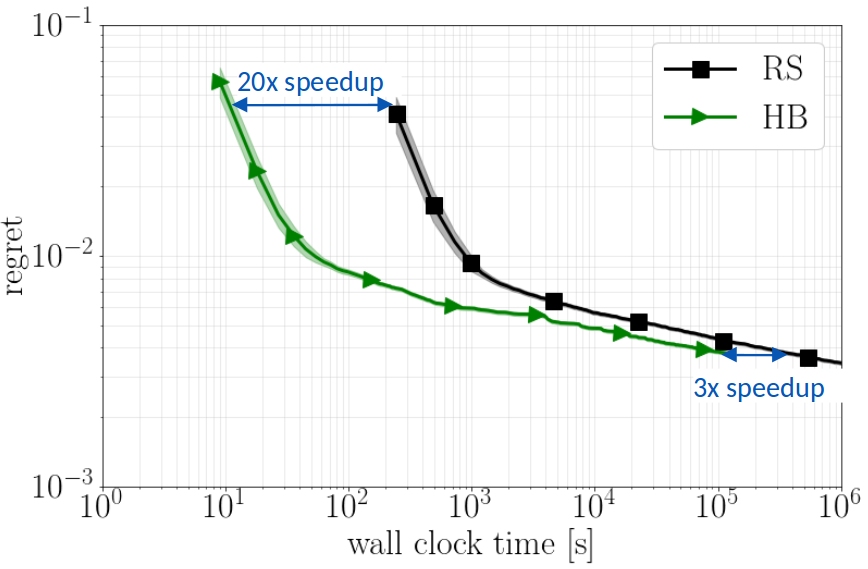
\includegraphics[width=\linewidth]{images/plots_aaron/bohb_2.png}
}

\myframe{Random search vs.\ Bayesian optimization}{
  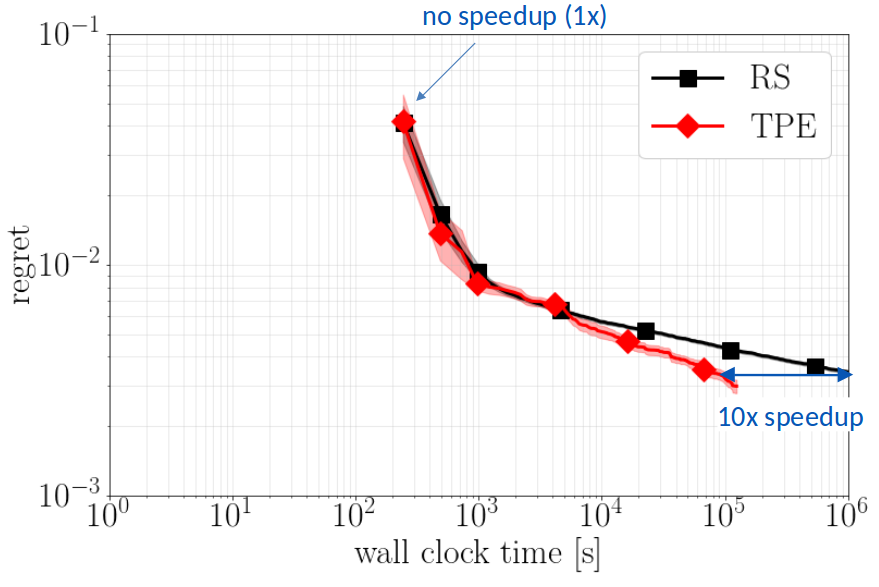
\includegraphics[width=\linewidth]{images/plots_aaron/bohb_1.png}
}

\myframe{BOHB achieves the best of both worlds}{
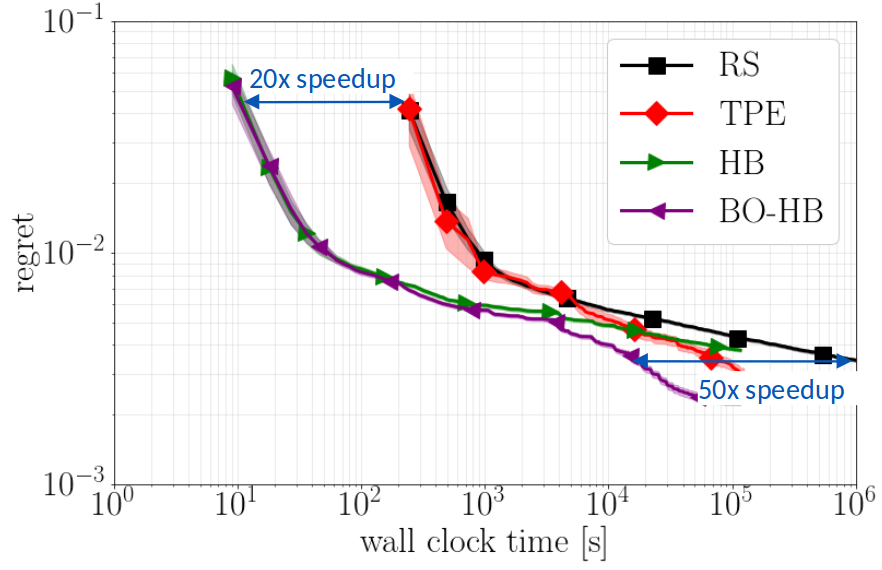
\includegraphics[width=\linewidth]{images/plots_aaron/bohb_3.png}
}









%-----------------------------------------------------------------------
%\begin{frame}[c,fragile]{Subset Selection \litw{Klein et al. 2017}}
%
%\begin{itemize}
%  \item Automatically choose dataset size for each evaluation
%  \item Include extra dimension in probabilistic model to capture dependence on dataset size s: $f(\lambda,s)$
%  \item Construct a second model for computational cost: $c(\lambda,s)$
%  \item Trade off information gain about global optimum vs. cost
%  \begin{itemize}
%   \item Entropy Search \lit{Hennig \& Schuler, JMLR 2012}:\\ Based on a probability distribution of where the maximum lies
%  \end{itemize} 
%\end{itemize}
%
%\centering
%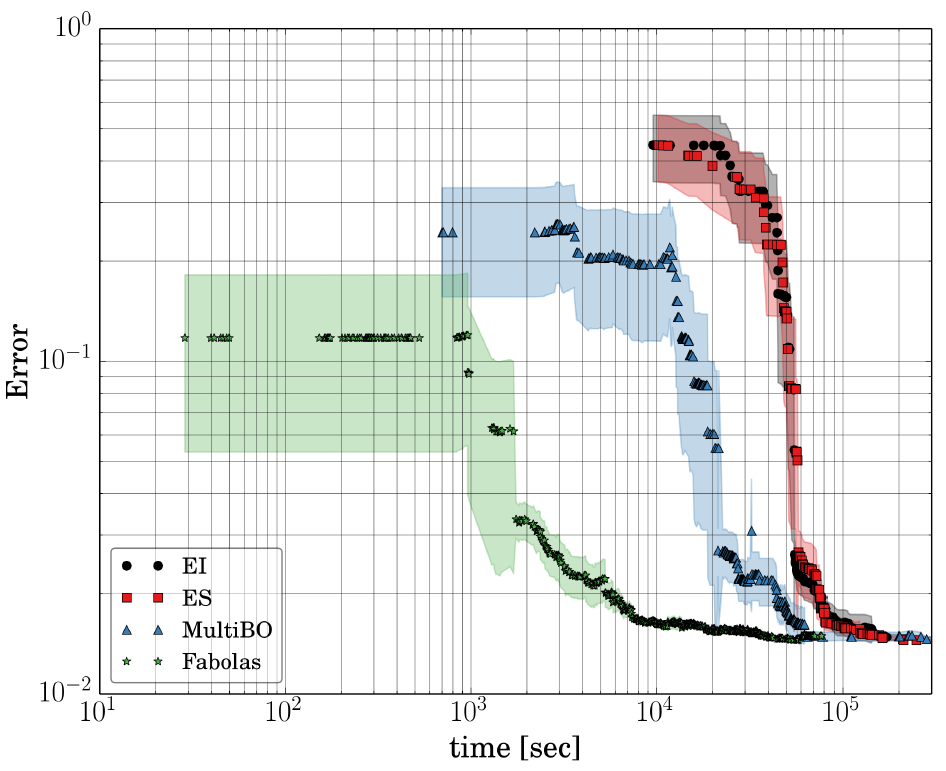
\includegraphics[width=0.4\textwidth]{images/subset_results}
%
%\end{frame}
%-----------------------------------------------------------------------

%-----------------------------------------------------------------------
%{\setbeamertemplate{logo}{}
%\begin{frame}[c,fragile]{Successive Halving \litw{Jamieson and Talwalkar 2015}}
%
%\begin{block}{Successive Halving}
%\begin{itemize}
%  \item Ideas: 
%  \begin{itemize}
%    \item Invest only resources in promising configurations
%    \item[$\leadsto$] aggressive dropping of poor configurations
%    \item Model-free --- (more or less assumption free)
%  \end{itemize}
%  \pause
%  \item Algorithm Outline:
%  \begin{enumerate}
%    \item[-] Input: $n$ (randomly sampled) configurations and budget $B$
%    \pause
%    \item Run remaining configurations with some resource allocation\\ (depending on $B$)
%%    \pause
%    \item Sort configurations by cost (e.$\,$g., validation loss)
%    \item Throw away lower half of configurations
%    \pause
%    \item Repeat
%  \end{enumerate}
%  \pause
%  \item Resource allocation can correspond to
%  \begin{itemize}
%    \item partial learning curves
%    \item subset of training data
%  \end{itemize}
%\end{itemize}
%\end{block}%
%
%\end{frame}
%}
%-----------------------------------------------------------------------
%-----------------------------------------------------------------------
%{\setbeamertemplate{logo}{}
%\begin{frame}[c,fragile]{Hyperband \litw{Li et al. 2016}}
%
%\begin{block}{Hyperband}
%\begin{itemize}
%  \item Issue of successive halving (for a fixed $B$):\\
%  		Do you want to run many configurations with aggressive rejection?\\
%  		Or: Do you want to run few configurations with non-aggressive rejection? 
%  \pause
%  \item Ideas: 
%  \begin{itemize}
%    \item Add an outer loop to try different trade-offs between $\#$configurations and budget
%    \item Add further parameter: proportion of configurations discarded in each round of successive halving
%  \end{itemize}
%  \pause
%  \item Starts with many configurations that gets aggressively rejected
%  \pause
%  \item In later iterations, few configurations with more budget each
%  \pause
%  \item Returns: configuration with the smallest intermediate loss seen so far.
%\end{itemize}
%\end{block}%
%
%\end{frame}
%}
%%-----------------------------------------------------------------------


%-----------------------------------------------------------------------
\section{Case Study: Auto-DispNet}
%-----------------------------------------------------------------------


%----------------------------------------------------------------------
\myframe{The Problem of Disparity Estimation}{
	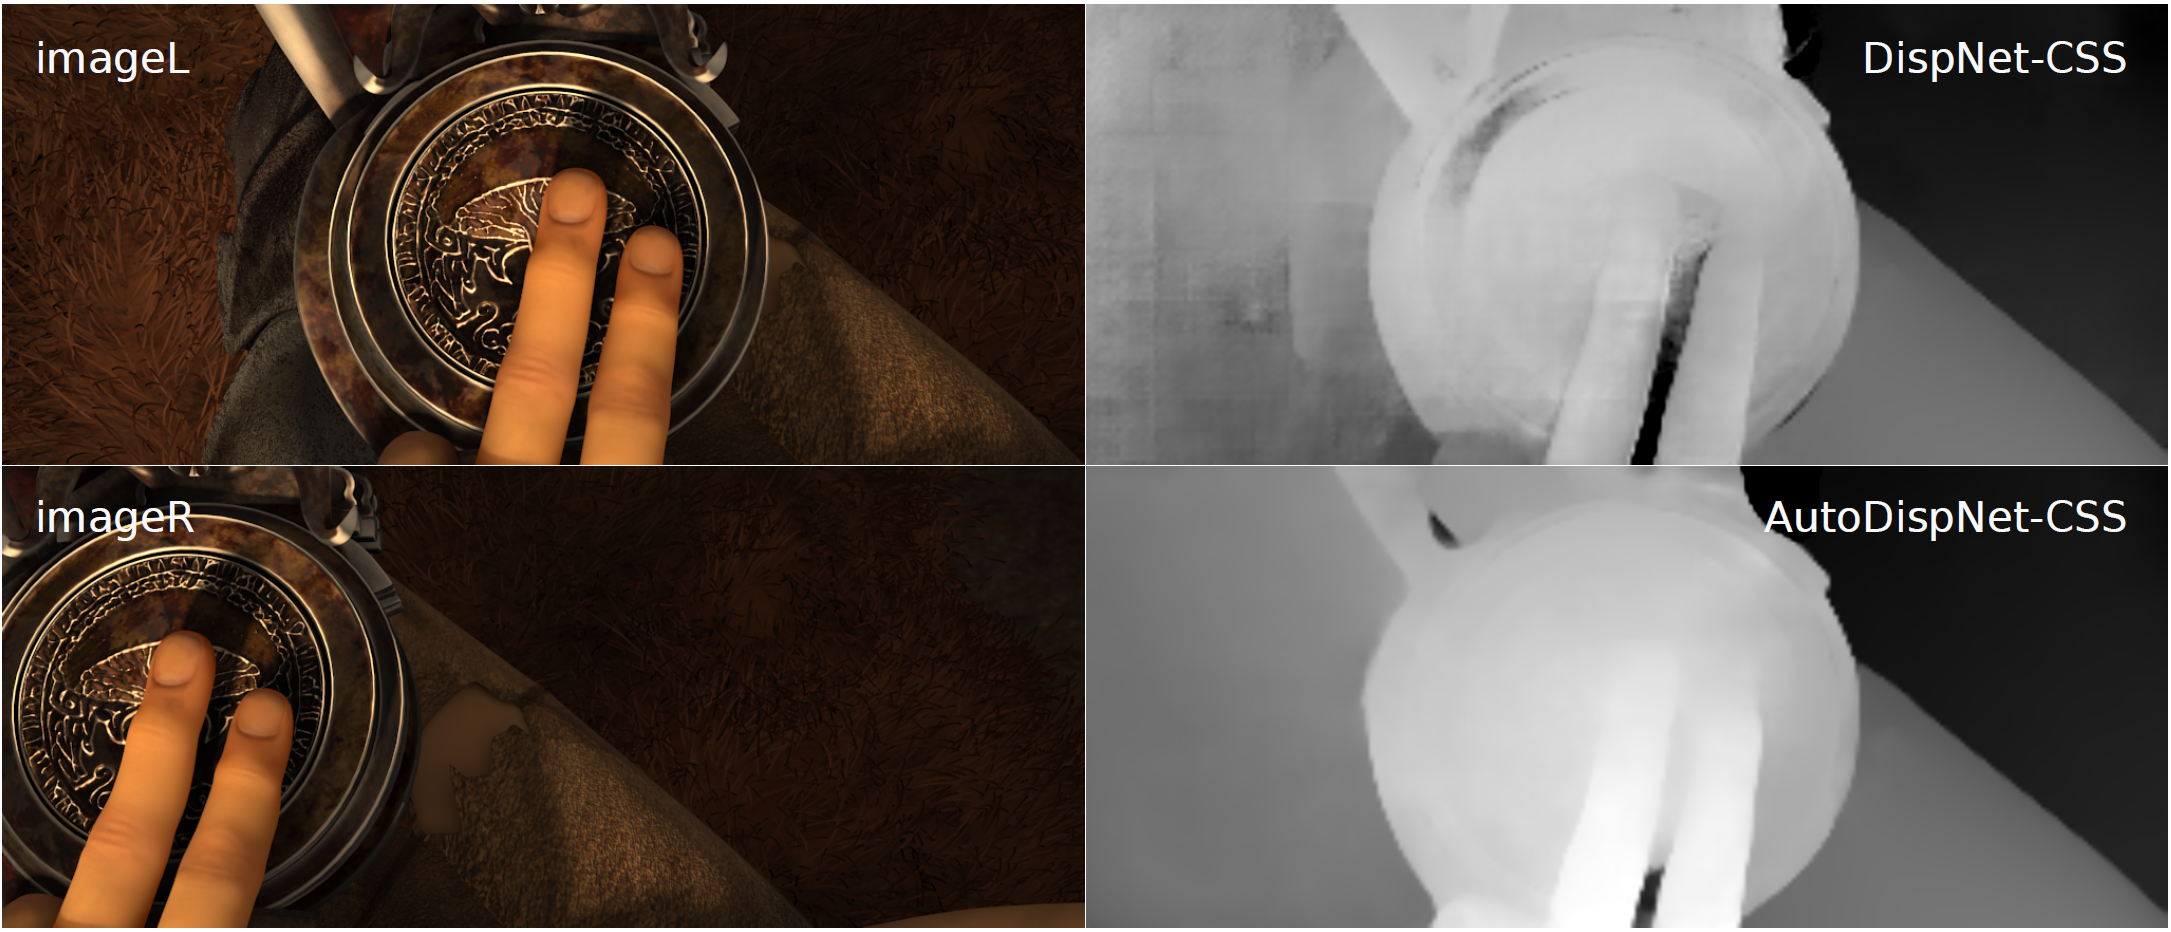
\includegraphics[width=\linewidth]{images_lec8/disparity_estimation}
}
%----------------------------------------------------------------------

%----------------------------------------------------------------------
\myframe{Background: U-Net}{
	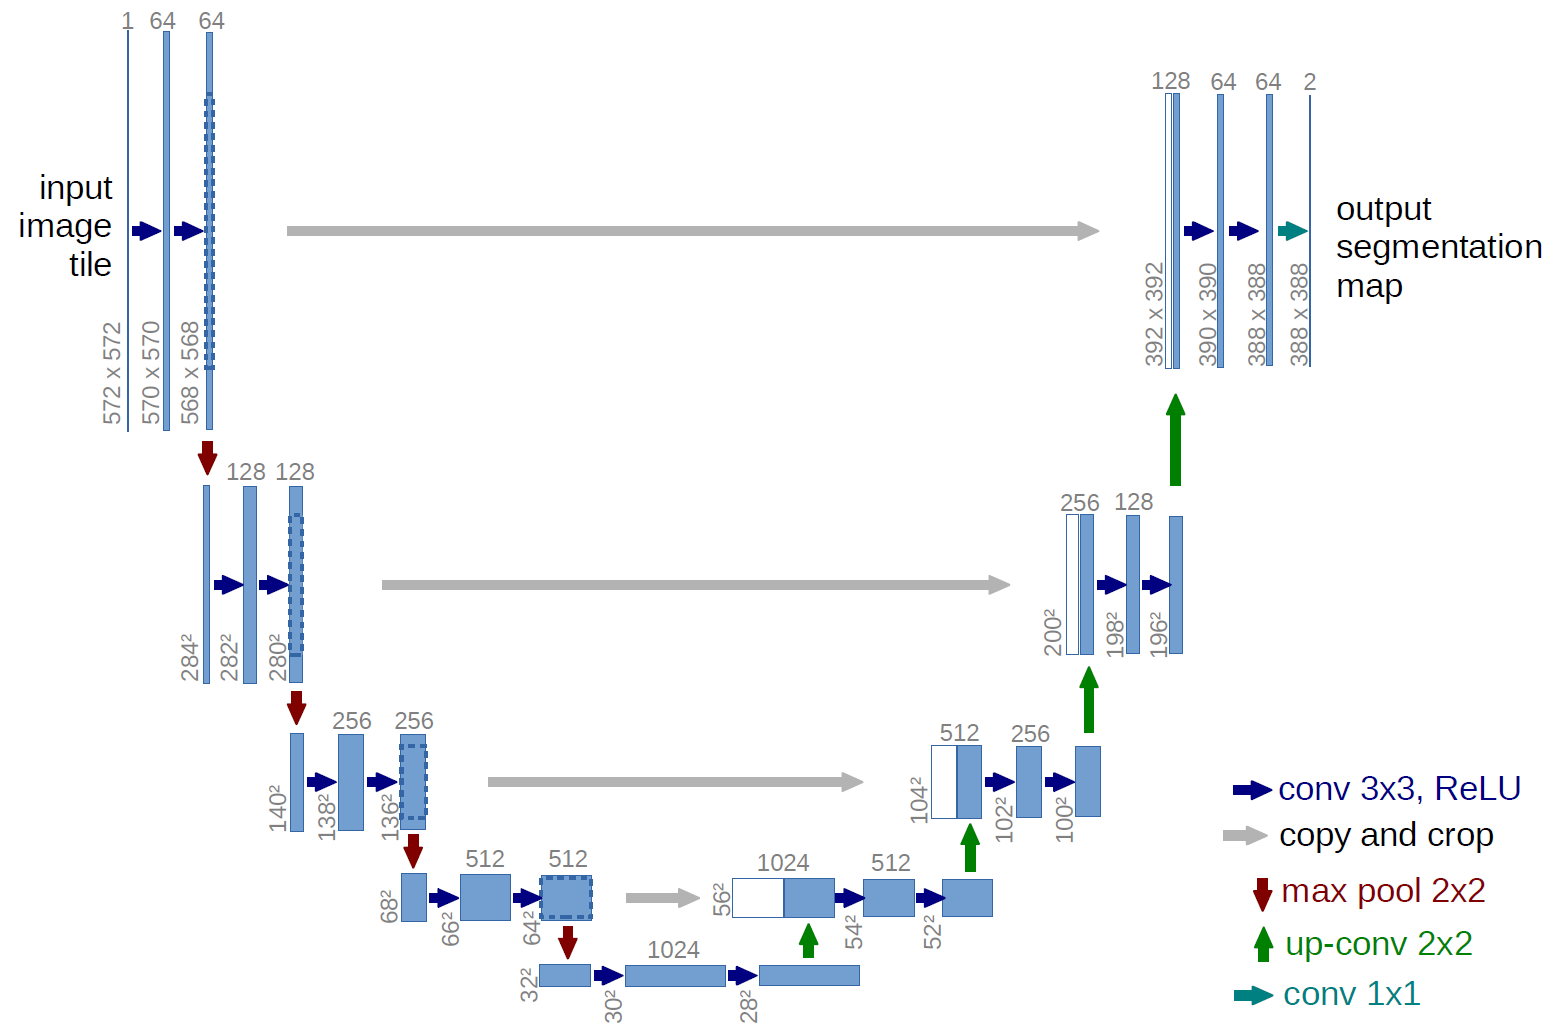
\includegraphics[width=0.85\linewidth]{images_lec8/u-net-architecture}
	\begin{center}
		\small{Skip connections from similar spatial resolution to avoid loosing information}	
	\end{center}	
}
%----------------------------------------------------------------------

%----------------------------------------------------------------------
\myframe{Search space}{
	\myit{
		\item Standard cells like in DARTS for 
		\myit{
			\item Keeping spatial resolution
			\item Downsampling
		}
		\item New upsampling cell that supports U-Net like skip connections 
	}	
\vspace*{0.3cm}
	\begin{center}
	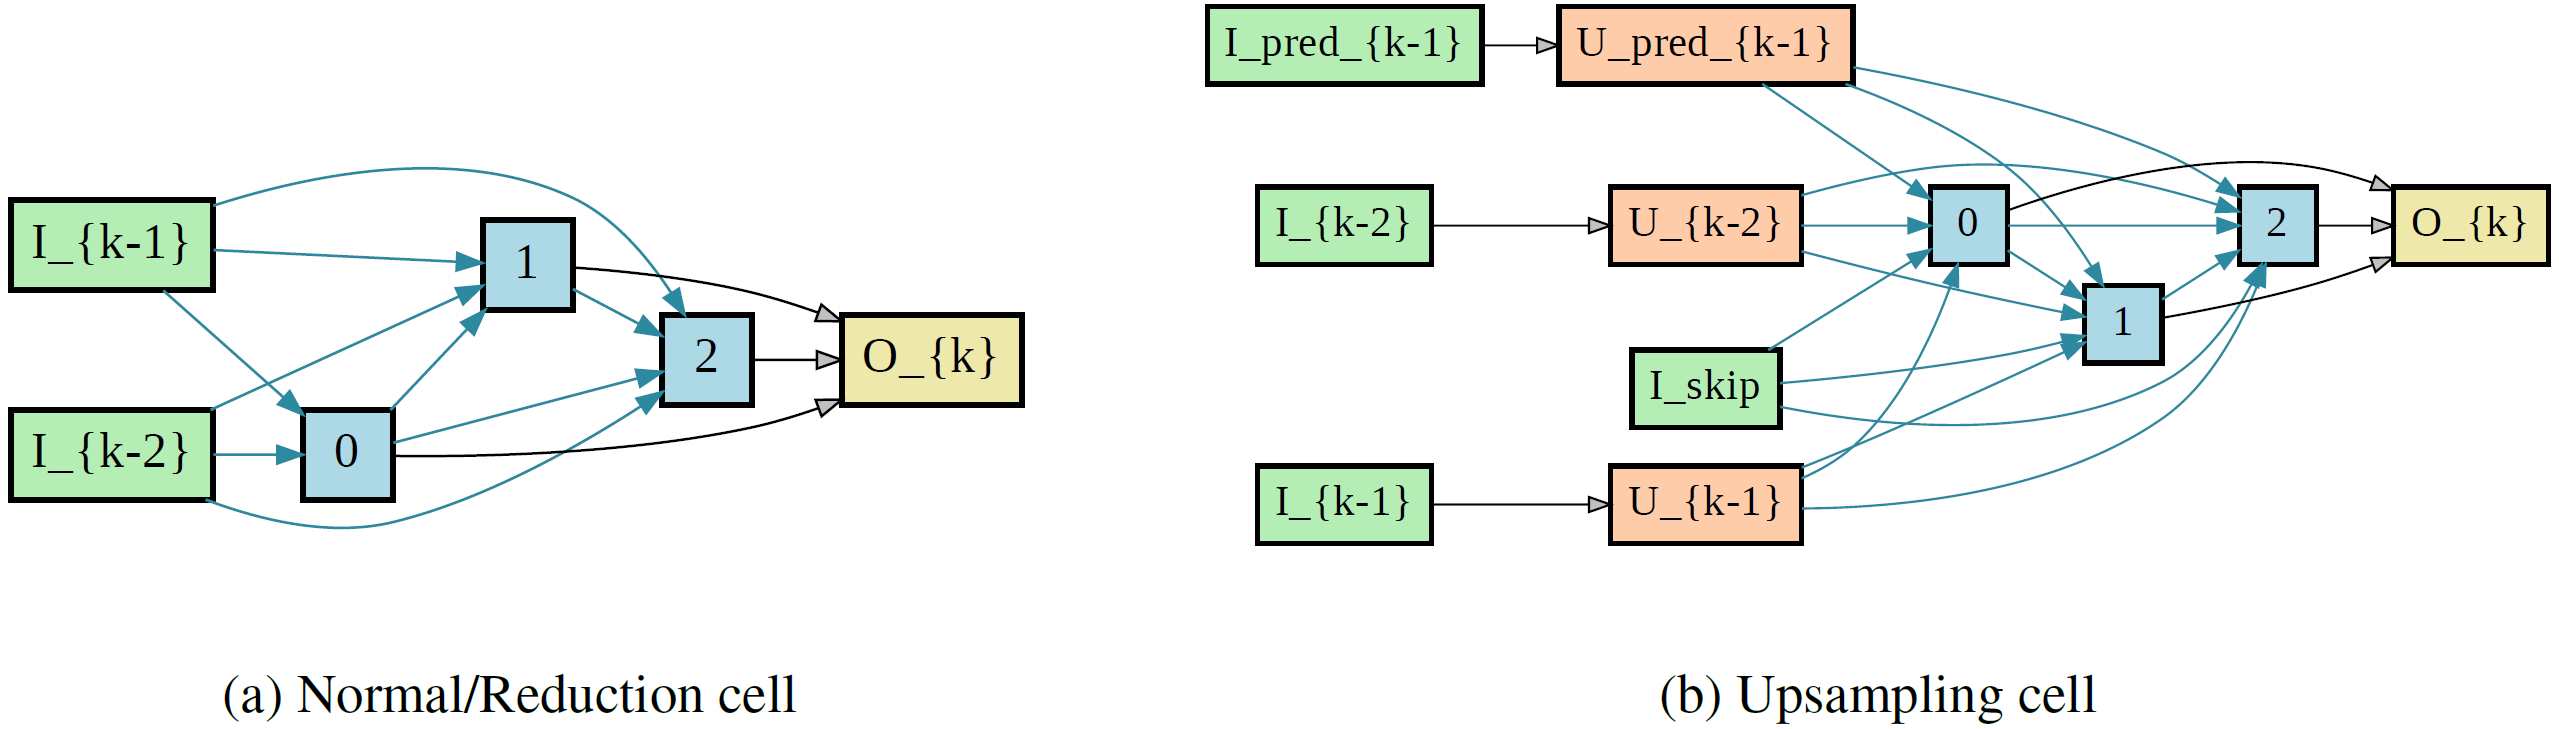
\includegraphics[width=0.85\linewidth]{images_lec8/cell_spaces_auto_dispnet}
	\end{center}
}
%----------------------------------------------------------------------

%----------------------------------------------------------------------
\myframe{Neural Architecture Search by DARTS, HPO by BOHB}{
	\myit{
		\item NAS: optimize neural architecture with DARTS
		\myit{
			\item Faster than BOHB
		}
		\medskip
		
		\item HPO: then optimize hyperparameters with BOHB
		\myit{
			\item DARTS does not apply
			\item The weight sharing idea is restricted to the architecture space
		}
		\medskip
		
		\item Result \lit{\href{https://arxiv.org/abs/1905.07443}{Saikat et al, 2019}}
		\myit{
			\item Both NAS and HPO yielded substantial improvements
			\item E.g., EPE on Sintel: \alert{2.36 $\rightarrow$ 2.14 $\rightarrow$ 1.94}
		}
	}	
}
%----------------------------------------------------------------------

%----------------------------------------------------------------------
\myframe{Details for Neural Architecture Search by DARTS}{
	\myit{
		\item Performance improved substantially
		\item Very important: \alert{warmstarting} of the network weights
		\myit{
			\item First, keep one-shot architecture weights fixed to the uniform distribution
			\item Only afterwards, alternative updates of weights and architectural parameters
		}
		\item Without warmstarting:\\
		\alert{DARTS found cells with only parameterless operations}
	}	
}
%----------------------------------------------------------------------

%----------------------------------------------------------------------
\myframe{Failure Modes of DARTS}{
	\begin{columns}
		\column{0.5\textwidth}
		\myit{
			\item Idenfified six small search spaces where DARTS fails badly\\ \lit{Zela et al, 2019}
			\item In all cases, it only selects skip connections 
	\medskip
	\medskip
	\medskip
			\item Overfitting of validation loss
			\item Can be fixed by more regularization:\\$L_2$ (for the inner objective), droppath, or early stopping
		}
		\column{0.5\textwidth}	
		\begin{center}
\vspace*{-0.2cm}
		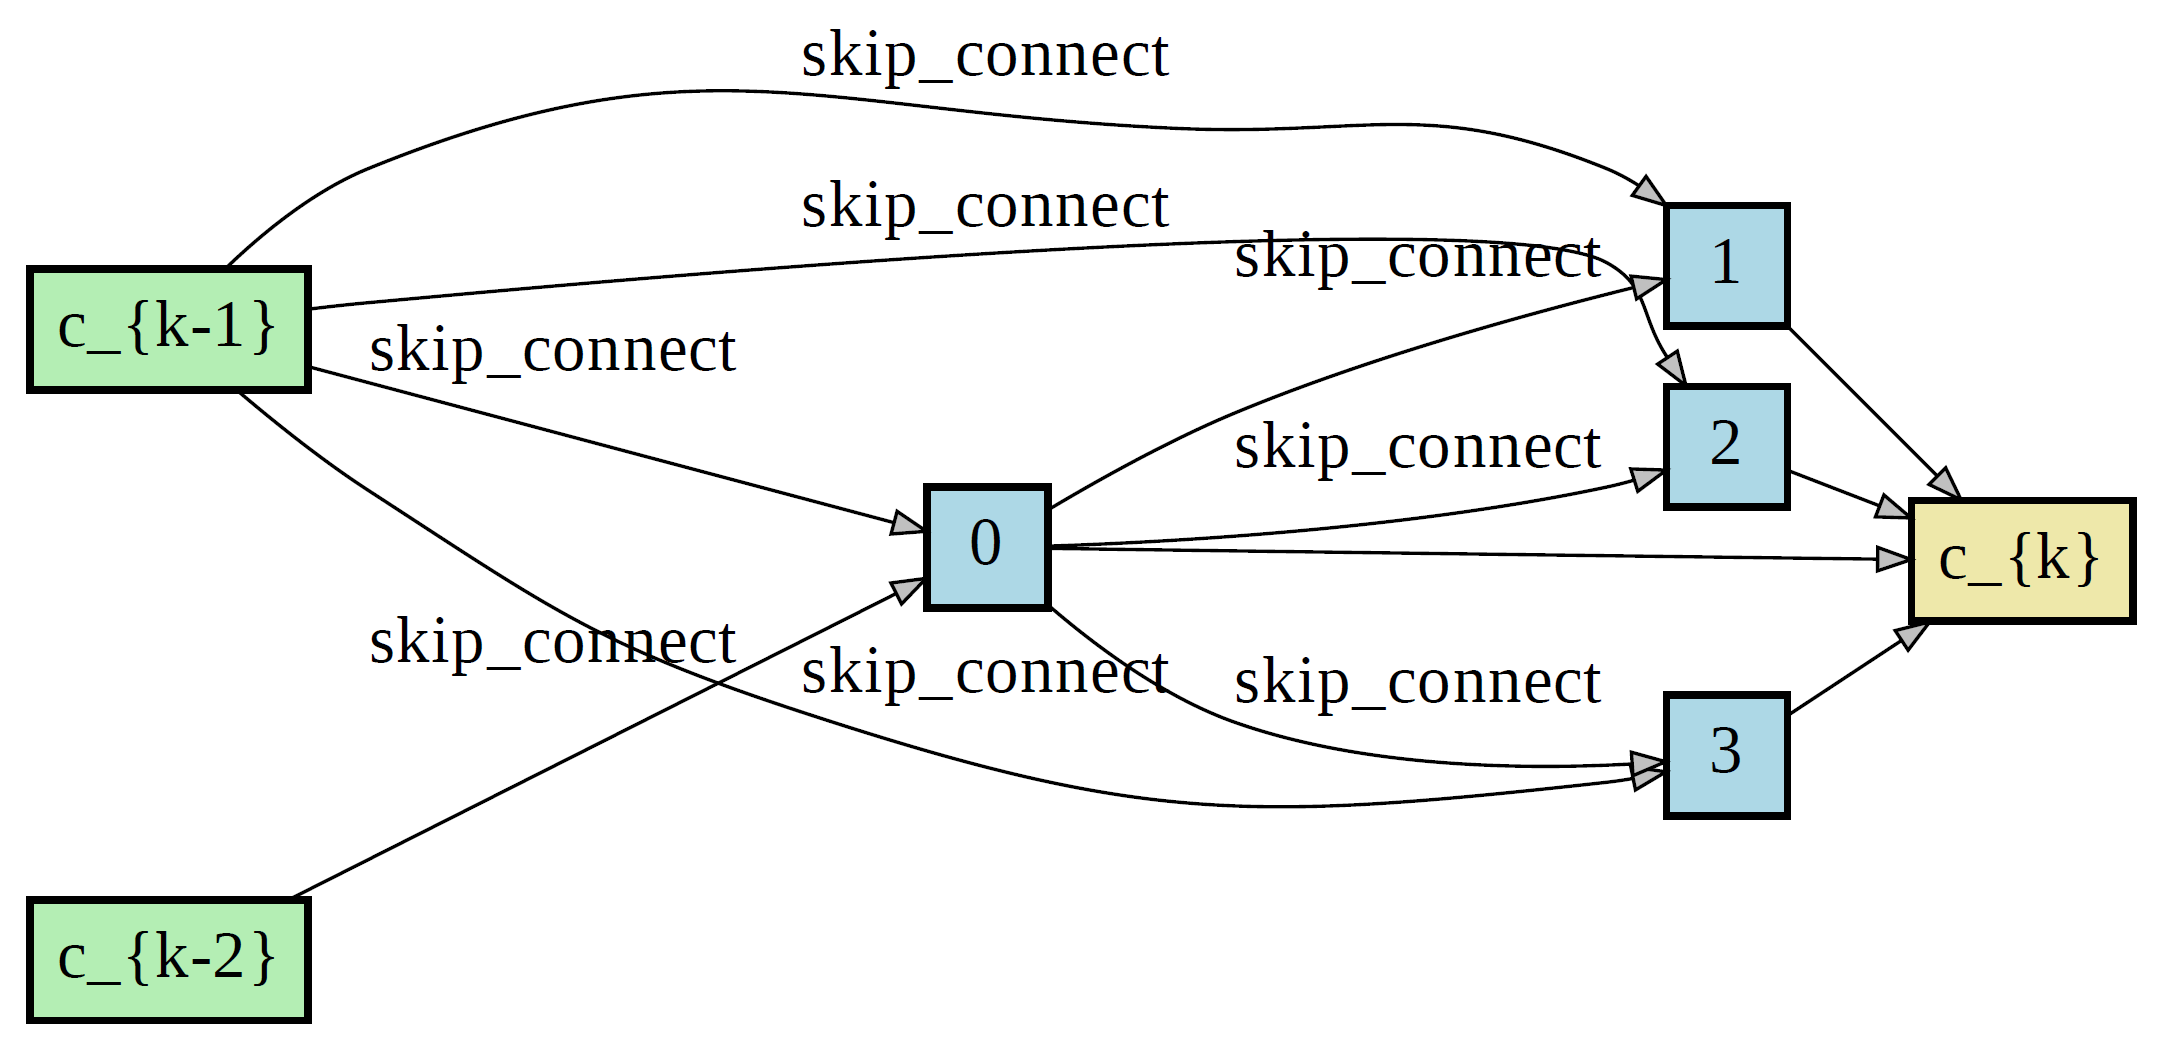
\includegraphics[width=0.9\linewidth]{images_lec8/DARTS_example_skip_connects}\\~\\
		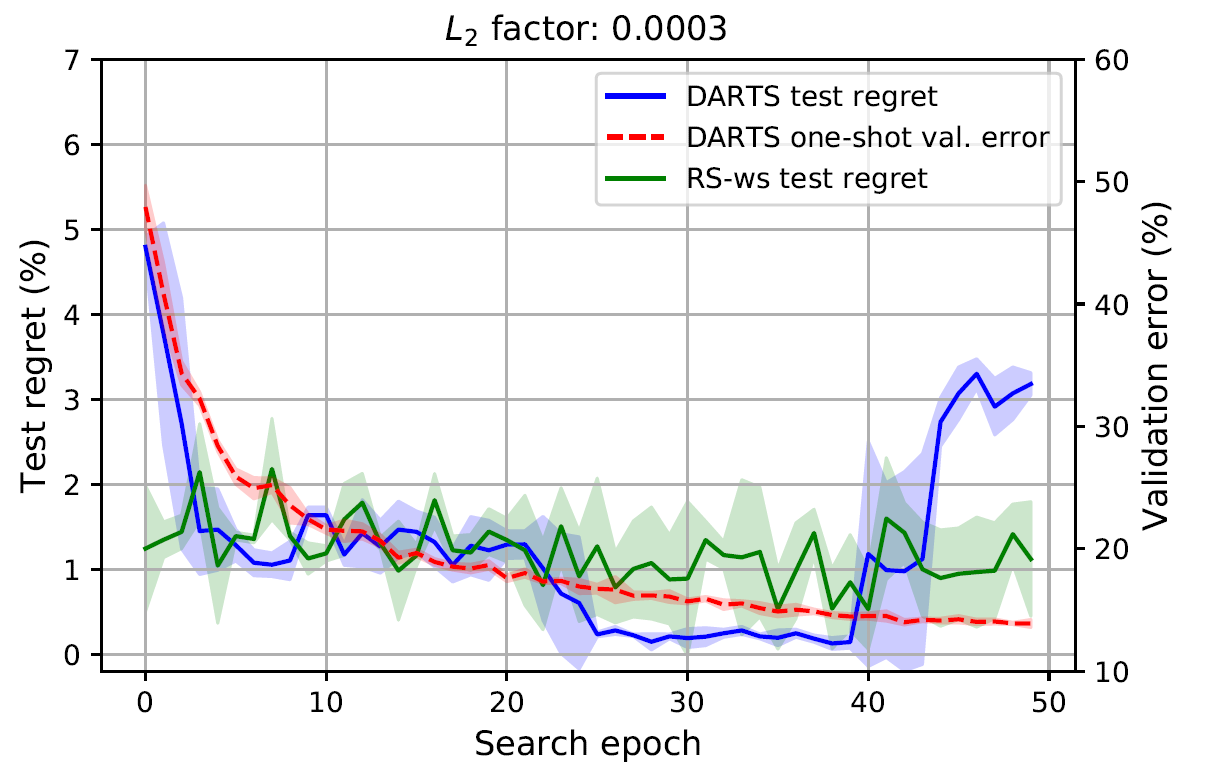
\includegraphics[width=0.9\linewidth]{images_lec8/DARTS_overfitting}
		\end{center}
	\end{columns}
}
%----------------------------------------------------------------------

%----------------------------------------------------------------------
\myframe{Recommendations for NAS and HPO}{
	\myit{
		\item So far, NAS often does not readily work out of the box
		\item BOHB typically does work out of the box
		\item Option 1: NAS, followed by HPO
		\item Option 2: Use HPO wrapped around NAS to make it more robust 
		\myit{
			\item Not evaluated so far, but likely good 
		}
	}
}
%----------------------------------------------------------------------




\section{NAS-Bench-101: Towards Reproducible Neural Architecture Search}

%-----------------------------------------------------------------------
\myframe{NAS-Bench-101}{
	\myit{
		\item Poor standards of research due to computational expense
		\item E.g., Zoph \& Le (2017) did not compare to other methods
		\myit{
			\item Spoiler: it turns out that Bayesian optimization with random forests (SMAC) is much better than RL
		}
\medskip		
		\item To fix this, we created a \alert{tabular surrogate benchmark}
		\myit{
			\item Small cell search space with 423k unique architectures for CIFAR-10
			\item Evaluated each of them \& stored result in a table
			\item Result: \alert{you can now quickly evaluate NAS algorithms on your laptop}
\medskip
			\item You can also run multi-fidelity algorithms 
			\myit{
				\item We evaluated for each of four different epoch budgets
				\item We also performed three repeats of each experiment
			}
		}
\medskip
		\item Just introduced, but already heavily taken up by the community
		\item Cannot evaluate weight sharing or weight inheritance algorithms
	}
}
%-----------------------------------------------------------------------

%-----------------------------------------------------------------------
\myframe{NAS-Bench-101: Search Space Details}{
	\rightimage[.4]{images_lec8/NAS-Bench-101-macro-space}
	\myit{
		\item \goleft[.45]{Cells are directed acyclic graphs with 3 operations:
		3x3 convolution, 1x1 convolution, 3x3 max-pool}
		\item \goleft[.45]{Limited number of vertices \& edges to limit to 423k models}
		\myit{
			\item \goleft[.45]{Maximum of 7 vertices, and 9 edges (out of 21)}
			\item \goleft[.45]{Architectures with $>9$ active edges are \alert{invalid}}
		}
	}
}
%-----------------------------------------------------------------------

%-----------------------------------------------------------------------
\myframe{NAS-Bench-101: Results}{
	\myit{
		\item Evaluated RL, regularized evolution (RE), random search (RS), Hyperband (HB), TPE, SMAC, BOHB	
		\item Test errors: RE, SMAC, BOHB $<$ RL $<$ RS \& HB
	}
	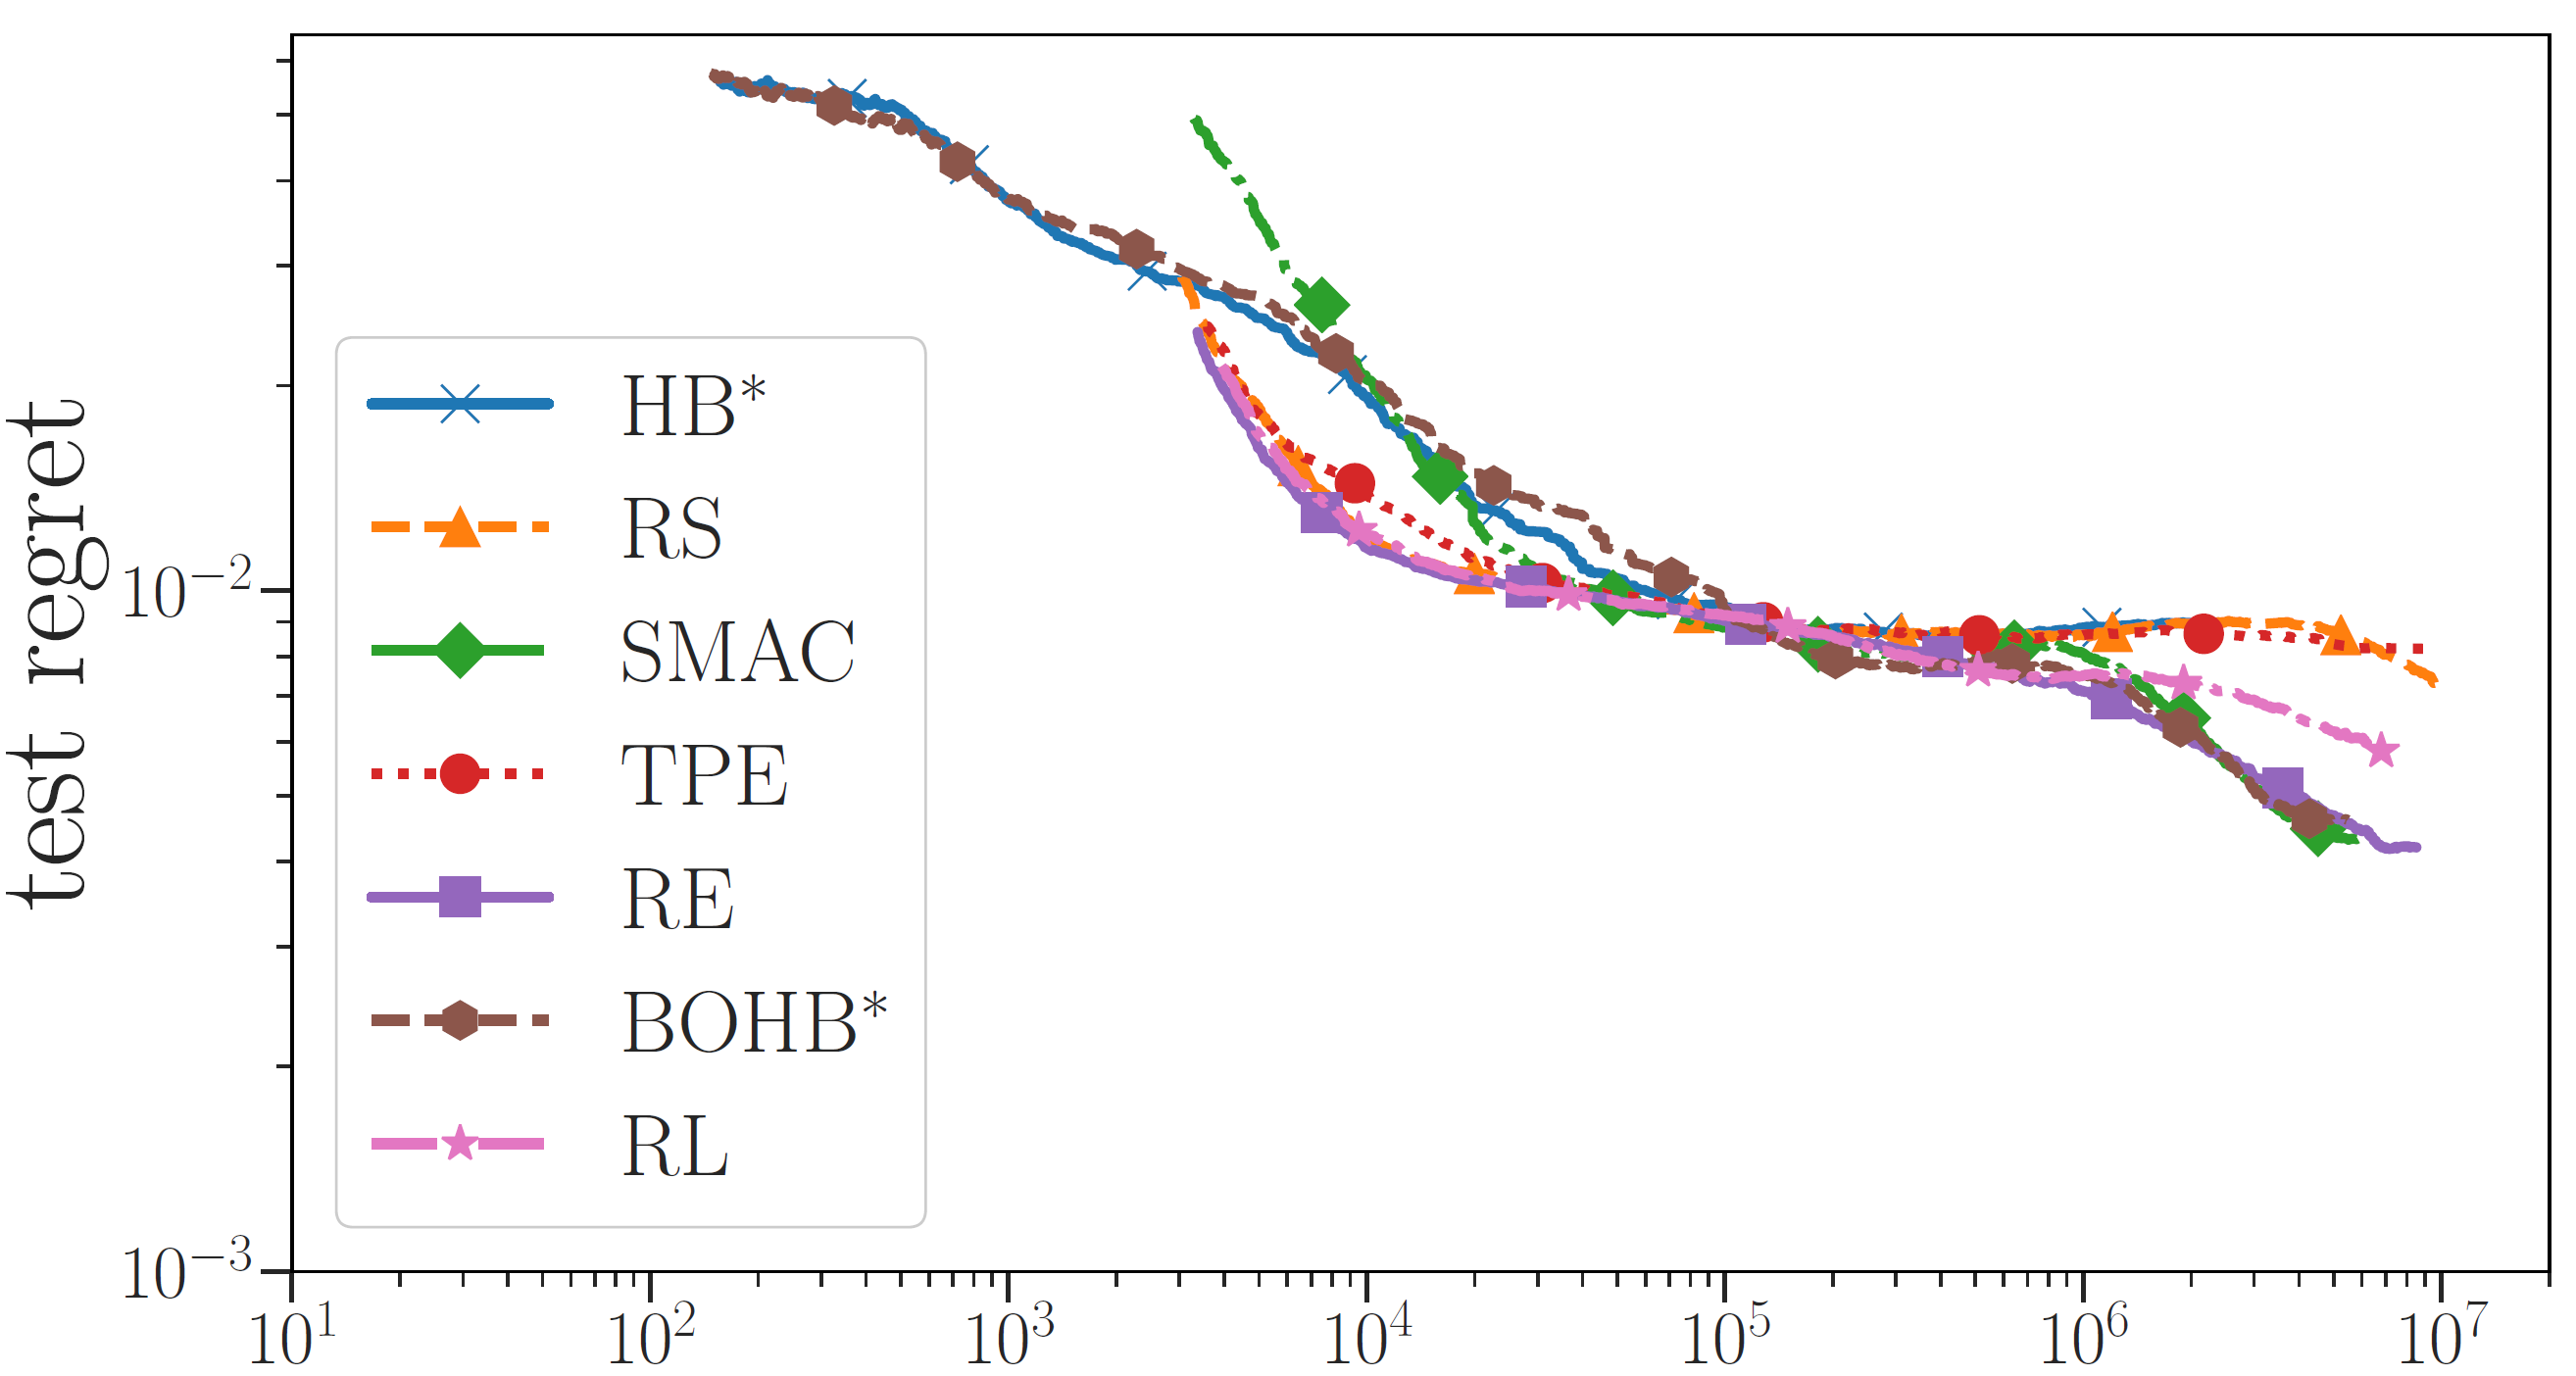
\includegraphics[width=0.9\linewidth]{images_lec8/NAS-Bench-101-results.png}
}
%-----------------------------------------------------------------------


%-----------------------------------------------------------------------
\myframe{Planned additional benchmarks}{
	\myit{
		\item \alert{Nas-Bench-201}
		\myit{
			\item Standard DARTS space, without any limitations
			\myit{
				\item Drop restriction to exhastive evaluations
				\item Only tiny fraction evaluated
				\item But 1M evaluations in, e.g., 50 dimensions, should make performance predictable
			}
			\item Include hyperparameters in the space $\rightarrow$ their choice is very important
			\item Pytorch instead of Tensorflow (thus probably not with Google)
		}
		\medskip
		\item \alert{HPOlib 2.0}
		\myit{
			\item Multi-fidelity benchmarks
			\item Multi-task benchmarks (several datasets)
		} 
	}
}
%-----------------------------------------------------------------------

%----------------------------------------------------------------------
\myframe{Learning Goals}{

	After this lecture, you will be able to \ldots
	
	\begin{itemize}
		\item describe \alert{several ways of speeding up over blackbox NAS}  %(except via meta-learning)
		\myit{
			\item define \alert{network morphisms} \& \alert{explain how to use them to speed up NAS}
			\item explain various \alert{methods for extrapolating learning curves}
			\item explain various \alert{multi-fidelity Bayesian optimization methods}
		}
		\item discuss \alert{when and how to use NAS and HPO in practice} 
		\myit{
			\item describe \alert{failure modes of DARTS}
			\item describe \alert{Auto-DispNet}
		} 
		\item describe \alert{NAS-Bench-101}, a benchmark for NAS
	\end{itemize}
}
